\documentclass[11pt]{article}
\usepackage{color}
\usepackage{nth}
\usepackage{enumitem}
\usepackage{booktabs}
\usepackage{tabularx}
\usepackage{hyperref}
\usepackage{placeins}
\usepackage[pdftex]{graphicx}
\usepackage{adjustbox}
\pagestyle{empty}
\setcounter{secnumdepth}{2}
\usepackage{float}
\usepackage{makeidx}
\makeindex
\usepackage{idxlayout}

\topmargin=0cm
\oddsidemargin=0cm
\textheight=22.0cm
\textwidth=17cm
\parindent=0cm
\parskip=0.15cm
\topskip=0truecm
\raggedbottom
\abovedisplayskip=3mm
\belowdisplayskip=3mm
\abovedisplayshortskip=0mm
\belowdisplayshortskip=2mm
\normalbaselineskip=12pt
\normalbaselines

% use case stuff
\newcounter{use case ID}

% environment slightly edited from https://tex.stackexchange.com/questions/10293/latex-template-for-use-cases
\newcommand\tabularhead[1]{
    \begin{table}[ht]
        \addtocounter{use case ID}{1}
        \caption{Use Case \arabic{use case ID} - #1}
        \vspace{0.2cm}
        \begin{tabular}{|p{0.2\linewidth}|p{0.70\linewidth}|}
            \hline
            \textbf{Action} & \textbf{#1} \\
            \hline}

        \newcommand\addrow[2]{#1 & #2\\ \hline}

            \newcommand\addmulrow[2]{ \begin{minipage}[t][][t]{2.5cm}#1\end{minipage}
                &\begin{minipage}[t][][t]{11cm}
                    \begin{enumerate}[itemsep=-1ex] #2   \end{enumerate}
                \end{minipage}\vfill\\ \hline}

            \newenvironment{usecase}{\tabularhead}
        {\hline\end{tabular}\end{table}}



        % cheaty non-functional requirement env

        \newcounter{req ID}
        \newcommand\tabularheadfsd[1]{
            \begin{table}[ht]
                \addtocounter{req ID}{1}
                \caption{Non-Functional Requirement \arabic{req ID} - #1}
                \vspace{0.2cm}
                \begin{tabular}{|p{0.2\linewidth}|p{0.70\linewidth}|}
                    \hline
                    \textbf{Action} & \textbf{#1} \\
                    \hline}

                \newenvironment{requirement}{\tabularheadfsd}
                {\hline\end{tabular}\end{table}}

                \begin{document}

                \vspace*{0.5in}
                \centerline{\bf\Large COMP 354}
                \centerline{\bf\Large Design document for 354TheStars}

                \vspace*{0.5in}
                \centerline{\bf\Large Group 5}

                \vspace*{0.5in}
                \centerline{\today}

                \begin{table}[htbp]
                    \caption{Group}
                    \begin{center}
                        \begin{tabular}{|r | c| c |}
                            \hline
                            Name & ID Number & Email \\
                            \hline
                            Morteza Ahmadi & 40038235 & morinob93@gmail.com \\
                            \hline
                            Mohd Tanvir & 40014010 & mohatanvir@hotmail.com \\
                            \hline
                            Arunraj Adlee & 40059206 & arunraj.adlee@hotmail.com \\
                            \hline
                            Dina Sadirmekova & 26321755 & dina.sadirmekova@gmail.com \\
                            \hline
                            Saima Syed & 40044790 & saima.syedb@gmail.com \\
                            \hline
                            Mehdi Skouri Saidi & 40057700 & mehdi879@hotmail.com \\
                            \hline
                            Trevor Lall & 40044047 & trevorlall95@gmail.com \\
                            \hline
                            Stefan John Bosco & 40057206 & johnboscostefan@gmail.com \\
                            \hline
                            Timothy Rodriguez & 40075447 & timmy\_258@hotmail.com \\
                            \hline
                            Lyonel Zamora & 27385986 & lyonelz516@gmail.com \\
                            \hline
                            Radhep Sabapathipillai & 40033092 & Radhep.Saba@gmail.com \\
                            \hline
                            Miguel Jimenez & 40022302 & migueleduardo298@hotmail.com\\
                            \hline
                        \end{tabular}
                    \end{center}
                \end{table}

                \begin{table}[htbp]
                    \caption{Revision history}
                    \begin{center}
                        \begin{tabular}{|r | c| c |}
                            \hline
                            Version & Date & Changes \\
                            \hline
                            1.0 & \nth{7} October 2019 & Completed requirements \\
                            \hline
                        \end{tabular}
                    \end{center}
                \end{table}
\clearpage

                \tableofcontents
\listoffigures
\clearpage
\listoftables

\clearpage

\section{Introduction}
\subsection{Purpose}
The software design document describes the architecture and system design of the online shopping website, 354TheStars. It includes use case diagrams and scenarios, an entity relation diagram, a class diagram, sequence diagrams, an architecture diagram, and screenshots of the external interface. It's intended to to communicate the design of the system to software developers and to coordinate its implementation.

\subsection{Scope}
354TheStars is planning to provide a worldwide platform, where various sized companies as well as individuals can sell or buy products. All of the available products shall be eligible for sale.

\subsection{Context}

Our system will mainly involve the user interacting with a web application interface. The user shall create an account to be able to buy or sell products, however user does not require to have an account for browsing the website. The user information will be stored in a remote database server. Users will not be able to create an account or login by using any social media platforms. It will be discussed in more details in future versions of this documentation.

\section{Use Cases}
\subsection{Selling}

The use case diagram below represents the Selling functionality of the 354TheStars Website. A detailed description of the "List items", "Sell items", and "Reply to reviews" use cases follows. The diagram reflects the added ability of the Seller to reply to reviews of their products. Only one reply per review is allowed and it doesn't include the ability to delete a review.

\begin{figure}[htbp]
    \centering
    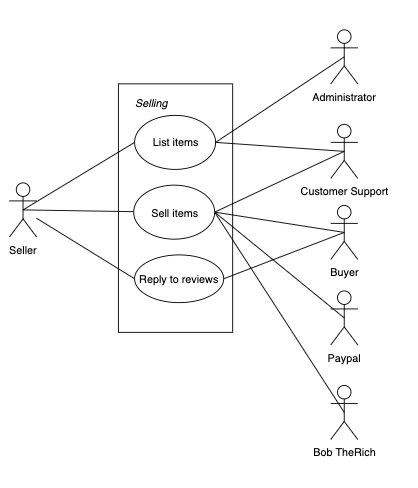
\includegraphics[width=0.5\textwidth]{Diagrams/Use_Case/ucdselling.png}
    \caption{Use Case Diagram 1: 354TheStars - Selling }
    \label{fig:ucd1}
\end{figure}

\begin{usecase}{List items}
    \addrow{Case ID}{UC01}
    \addrow{Actors}{\textbf{Seller, Administrator, Customer Support}}
    \addrow{Summary}{\index{seller}Seller completes all the \index{information}information necessary to list an item and has the option to edit or delete it. The \index{administrator}Administrator can manage all the listings information. In case of any issues, the Customer Support can be contacted.}
    \addrow{Pre-Conditions}{The user is registered as a legitimate seller.}
    \addrow{\index{data}Data}{Product photo, \index{product}product description, price, stock count,product name,category.}
    \addrow{Stimulus}{Seller pressed on Add Listing/Edit Listing/Delete Listing Button}
    \addmulrow{Response}{
            \item Add Listing/Edit Listing/Delete Listing dialogue appears.
            \item \index{seller}Seller fills out all the information.
            \item Listing added/edited/deleted successfully.
    }
    \addmulrow{Exceptions}{
            \item The required information is not filled out.
            \item The description is over the character limit (100 characters).
    }
    \addrow{Priority}{High}
    \addmulrow{Open Issues}{
            \item Should the \index{seller}Seller be able to preview the listing?
            \item What happens if the item is illegal?
            \item How do we check the quality of the image?
            \item How do we check if the seller is legitimate?
    }
\end{usecase}


\begin{usecase}{Sell items}
    \addrow{Case ID}{UC02}
    \addrow{Actors}{\textbf{Seller, Buyer, PayPal, Bob TheRich, Customer Support}}
    \addrow{Summary}{Seller accepts \index{payment}payment for the item from \index{buyer}Buyer and pays Bob TheRich the 8\% of the sale fee.
    However,for the first 10 items sold by the seller, Bob TheRich gets only 3\% to encourage new sellers. The \index{seller} Seller and Bob TheRich can access the sales history. In case of any issues, the Customer Support can be contacted.}
    \addrow{Pre-Conditions}{Seller, \index{buyer}Buyer, and Bob TheRich must have a valid \index{PayPal}PayPal account. }
    \addrow{\index{data}Data}{PayPal account \index{information}information, sales \index{data}data, 3\% fee for first 10 items 8\% afterwards, shipped items}
    \addrow{Stimulus}{Buyer paid for item(s)}
    \addmulrow{Response}{
            \item \index{PayPal}PayPal transfers money from the \index{buyer}Buyer account to the Seller Account and sends a confirmation.
            \item \index{seller}Seller receives a sale notification by email.
            \item The sale appears in the Seller’s sales history.
            \item Bob TheRich invoices the Seller for 3\% if this is the sellers first 10 items,otherwise the invoice is of 8\%.
            \item Seller pays Bob TheRich through PayPal.
            \item Seller marks item as shipped.
    }

    \addmulrow{Exceptions}{
            \item Confirmation from \index{PayPal}PayPal not received.
    }
    \addrow{Priority}{High}
    \addmulrow{Open Issues}{
            \item What happens if the sale appears in the sales history but not in the shipped items history after a predetermined amount of time?
    }
\end{usecase}

\begin{usecase}{Reply to reviews}
    \addrow{Case ID}{UC03}
    \addrow{Actors}{\textbf{Seller}}
    \addrow{Summary}{\index{seller}Seller is able to reply to a review left by a buyer.}
    \addrow{Pre-Conditions}{The user is registered as a legitimate seller. }
    \addrow{\index{data}Data}{Product photo, seller's username.}
    \addrow{Stimulus}{Seller hits the reply button to a buyer's review.}
    \addmulrow{Response}{
            \item Seller replies to the buyer.
            \item Seller can add a picture(optional)
            \item The reply is displayed under the buyers review.
            \item Reply is visible to everyone.
    }
    \addmulrow{Exceptions}{
            \item The seller already replied to the buyer (Cannot reply more than once)
            \item The reply is over the character limit (400 characters).
    }
    \addrow{Priority}{Medium}
    \addmulrow{Open Issues}{
        \item Can the seller preview his message before posting?
        \item Should the buyer receive a notification when the seller replies?
        \item How are we handling offensive replies?
    }
\end{usecase}

\clearpage

\subsection{Buying}

The use case diagram below represents the Buying functionality of the Online Shopping Website. A detailed description of each use case follows.

\begin{figure}[htbp]
    \centering
    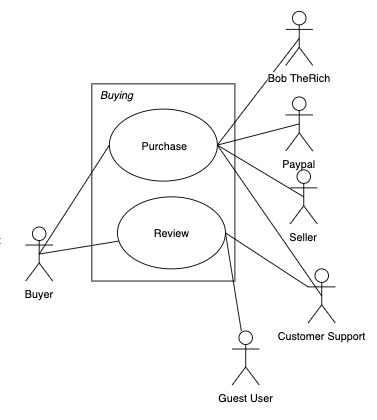
\includegraphics[width=0.5\textwidth]{Diagrams/Use_Case/ucd2.png}
    \caption{Use Case Diagram 2: Online Shopping Website - Buying }
    \label{fig:ucd2}
\end{figure}

\begin{usecase}{Purchase}
    \addrow{Case ID}{UC04}
    \addrow{Actors}{\textbf{Buyer, Seller, PayPal, Bob TheRich, Customer Support}}
    \addrow{Summary}{The Buyer views the shopping cart, has the option to modify it, and pays for it. In case of any issues, the Customer Support can be contacted.}
    \addmulrow{Pre-Conditions}{
        \item \index{buyer}Buyer is a \index{registered user}registered user.
        \item Buyer has a valid \index{PayPal}PayPal account.
        \item \index{seller}Seller contact information is hidden.
    }
    \addrow{\index{data}Data}{Purchase photo, purchase description, purchase quantity, purchase price per item, total purchase price, taxes, shipping fee, shipping address, PayPal account, \index{receipt}receipt (Seller \index{information}information, Buyer information, purchase date, purchase details, purchase price, taxes)}
    \addrow{Stimulus}{Buyer presses the Checkout Button.}
    \addmulrow{Response}{
            \item \index{buyer}Buyer views the shopping cart information and can modify it.
            \item Buyer chooses the shipping option (standard or express).
            \item Buyer chooses the shipping address.
            \item Buyer pays the \index{seller}Seller for the purchase through \index{PayPal}PayPal.
            \item A confirmation screen is displayed.
            \item Buyer receives a confirmation and \index{receipt}receipt by email.
            \item Order added to the purchase history.
    }
    \addmulrow{Exceptions}{
        \item Any of the required \index{information}information is missing or incorrect
        \item \index{buyer}Buyer exceeded the time limit to complete purchase
        \item Buyer abandons the cart
        \item The confirmation screen is not displayed
    }
    \addrow{Priority}{High}
    \addmulrow{Open Issues}{
        \item What happens if the \index{buyer}Buyer is not allowed to purchase the \index{product}product legally?
    }

\end{usecase}

\begin{usecase}{Review}
    \addrow{Case ID}{UC05}
    \addrow{Actors}{\textbf{Buyer, Guest User, Customer Support}}
    \addrow{Summary}{\index{buyer}Buyer leaves a \index{review}review for a product previously purchased. In case of any issues, the Customer Support can be contacted.}
    \addrow{Pre-Conditions}{
        15 days must have passed since the \index{buyer}Buyer’s purchase of the \index{product}product being reviewed.
        }
    \addrow{\index{data}Data}{
Review text, \index{review}review photo, days since purchase, Buyer’s username, rating (out of 5 stars)
}
    \addrow{Stimulus}{Buyer clicks on the Add Review button}
    \addmulrow{Response}{
        \item \index{buyer}Buyer rates the \index{product}product
        \item Buyer adds \index{review}review text
        \item Buyer adds review photos (optional)
        \item Buyer posts the review
        \item Review appears on the product page for any \index{guest user}Guest User to view
    }
    \addmulrow{Exceptions}{
        \item 15 days haven’t passed since the purchase
        \item Buyer posted more than 5 photos per \index{review}review
        \item Review over the character limit (400 characters)
        \item Any of the required \index{information}information is missing
    }
    \addrow{Priority}{Medium}
    \addmulrow{Open Issues}{
        \item Should the \index{buyer}Buyer be able to preview the review?
        \item How do we handle offensive \index{review}reviews?
    }
\end{usecase}


\clearpage
\subsection{Login}

The use case diagram below represents the login functionality of the Online Shopping Website. A detailed description of each use case follows.

\begin{figure}[htbp]
    \centering
    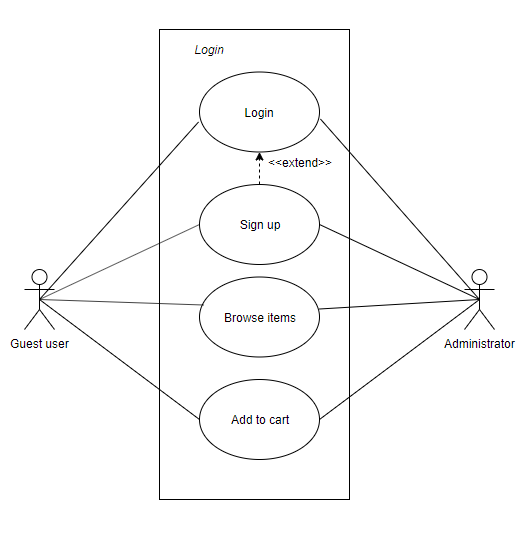
\includegraphics[width=0.5\textwidth]{Diagrams/Use_Case/ucd3.png}
    \caption{Use Case Diagram 3: Online Shopping Website - Login }
    \label{fig:ucd3}
\end{figure}

\begin{usecase}{Login}
    \addrow{Case ID}{UC06}
    \addrow{Actors}{\textbf{Guest user, Administrator}}
    \addrow{Summary}{Any \index{guest user}guest user can sign in to their account. Same goes for the \index{administrator}administrator.}
    \addmulrow{Pre-Conditions}{
        \item Must have an existing account
    }
    \addrow{\index{data}Data}{Username and password}
    \addrow{Stimulus}{\index{guest user}Guest user presses the login button.}
    \addmulrow{Response}{
            \item User will have the option to sell \index{product}products.
            \item User will have the option to buy products.
            \item User can browse and put items in his cart.
            \item \index{administrator}Administrator will have access to private \index{information}information.
            \item Administrator will be able to manege the website.
    }
    \addmulrow{Exceptions}{
        \item Username and/or password incorrect.
    }
    \addrow{Priority}{High}
    \addmulrow{Open Issues}{
        \item What if the \index{guest user}guest user forgets his/her password or username?
        \item Is there a limit of attempt for safety reason ?
    }

\end{usecase}

\begin{usecase}{Signup}
    \addrow{Case ID}{UC07}
    \addrow{Actors}{\textbf{Guest user, Administrator}}
    \addrow{Summary}{The \index{administrator}administrator and the \index{guest user}guest user should be able to create an account at any time.}
    \addrow{Pre-Conditions}{
       User has an email address.
        }
    \addrow{\index{data}Data}{
username, password, address, email, phone number
}
    \addrow{Stimulus}{\index{guest user}Guest user presses the sign up button}
    \addmulrow{Response}{
        \item user will have to fill out a formula.
        \item user will enter his/her personal \index{information}information.
        \item user will have access to more features.
    }
    \addmulrow{Exceptions}{
        \item User doesn't enter correct \index{information}information.
        \item Username taken/password weak.
    }
    \addrow{Priority}{High}
    \addmulrow{Open Issues}{
        \item What if the user already have an account and creates another one?
        \item How are we verifying that no two user have the same username?
        \item For security reasons,how are we handling weak passwords?
    }
\end{usecase}

\begin{usecase}{Browse item}
    \addrow{Case ID}{UC08}
    \addrow{Actors}{\textbf{Guest user, Administrator}}
    \addrow{Summary}{Both user can browse the items through the website and/or search for a specific item.}
    \addrow{Pre-Conditions}{
       None , anyone can browse.
        }
    \addrow{\index{data}Data}{
    item name, item description,item price}
    \addrow{Stimulus}{User writes on the search bar or use the drop down menu to filter item by category. }
    \addmulrow{Response}{
        \item the page will load all the items related.
        \item The page will display the names and thumbnails of each item.
    }
    \addmulrow{Exceptions}{
        \item item not found (does not exist)
    }
    \addrow{Priority}{High}
    \addmulrow{Open Issues}{
        \item How are we handling spelling errors (ex;show suggestions) ?
    }
\end{usecase}



\begin{usecase}{Add to cart}
    \addrow{Case ID}{UC09}
    \addrow{Actors}{\textbf{Guest user, Administrator}}
    \addrow{Summary}{Whenever a user sees something that they like, they can put that item in their cart to eventually buy.}
    \addrow{Pre-Conditions}{
       Must be a \index{registered user}registered user.
        }
    \addrow{\index{data}Data}{
item picture, price of item, name of the \index{seller}seller,total price of all items chosen,quantity of each item chosen.}
    \addrow{Stimulus}{User click a button to add an item to his/her cart.}
    \addmulrow{Response}{
        \item The item will appear in the user's cart.
        \item The user will be able to go look at the cart.
        \item The user will be able to remove an item or continue adding.
    }
    \addmulrow{Exceptions}{
        \item Item is out of stock.
    }
    \addrow{Priority}{High}
    \addmulrow{Open Issues}{
        \item What happens to the cart if it contains items and the user exit the website?
    }
\end{usecase}
\clearpage


\subsection{Admin Panel}

The use case diagram below represents the Admin Panel functionality of the 354TheStars website. A user of the admin type should be able to login to his admin account. From there, the admin should be able to create, delete, modify user accounts. He should be able to view user information. The admin should also be able to view, delete, modify all user listings. Moreover, the admin has the ability to view and delete any reviews, and add or remove product categories. As specified in the new requirements, the Admin Panel allows the admin to generate site activity reports such as a list of sellers ranked by the number of items sold during a specified period of time. The admin is also responsible for the website maintenance. He should be able to keep the website functional at all times, ensure the security of the system, and the quality of the database.

\begin{figure}[htbp]
    \centering
    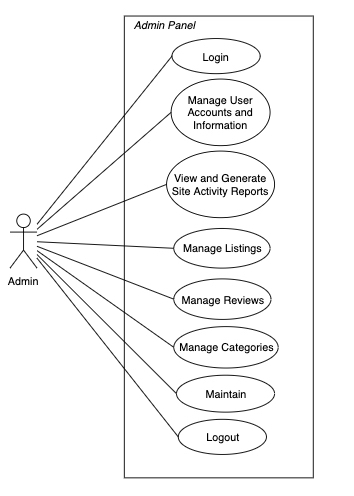
\includegraphics[width=0.5\textwidth]{Diagrams/Use_Case/ucdadmin.png}
    \caption{Use Case Diagram 4: 354TheStars - Admin Panel }
    \label{fig:ucd4}
\end{figure}

\clearpage
\subsection{Site Browsing}

The use case diagram below represents the Site Browsing functionality of the 354TheStars website. It demonstrates how the guest users, and clients will interact with the interface of the site when browsing for items. Displaying listings is how users will be able to view what items the site provides. They will also be recommended products, have the ability to filter the listings and search for items with the interface. Furthermore, users will be able to add items to their cart when they are ready to purchase them, as well as view what items exists in their cart already. Clients that are signed up with the site will be able to view their account information, as well as login and logout of the site. Guest users will be able to register when they click on view account. Lastly, the site will generate advertisements and will be able to generate specific ads based on a user's cookie history. Bob the rich and advertisers make money with this implementation via ad revenue.

\begin{figure}[htbp]
    \centering
    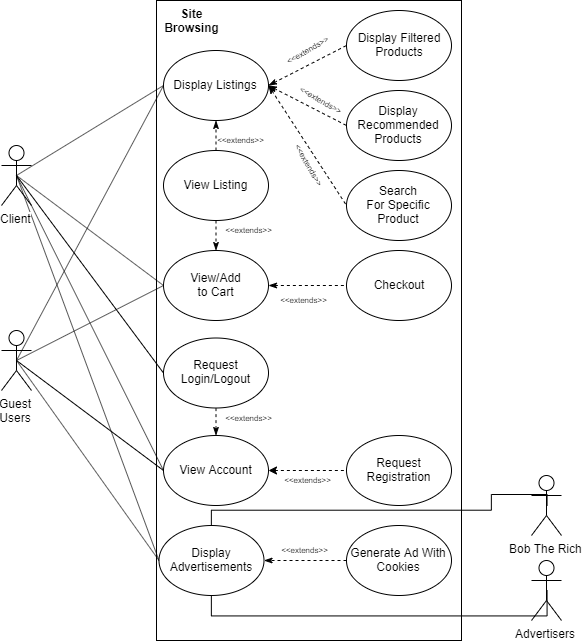
\includegraphics[width=0.65\textwidth]{Diagrams/Use_Case/ucd4.png}
    \caption{Use Case Diagram 5: 354TheStars - Browsing }
    \label{fig:ucd5}
\end{figure}


\clearpage
\section{Entity Relationship Diagram}
\begin{figure}[ht!]
    \centering
    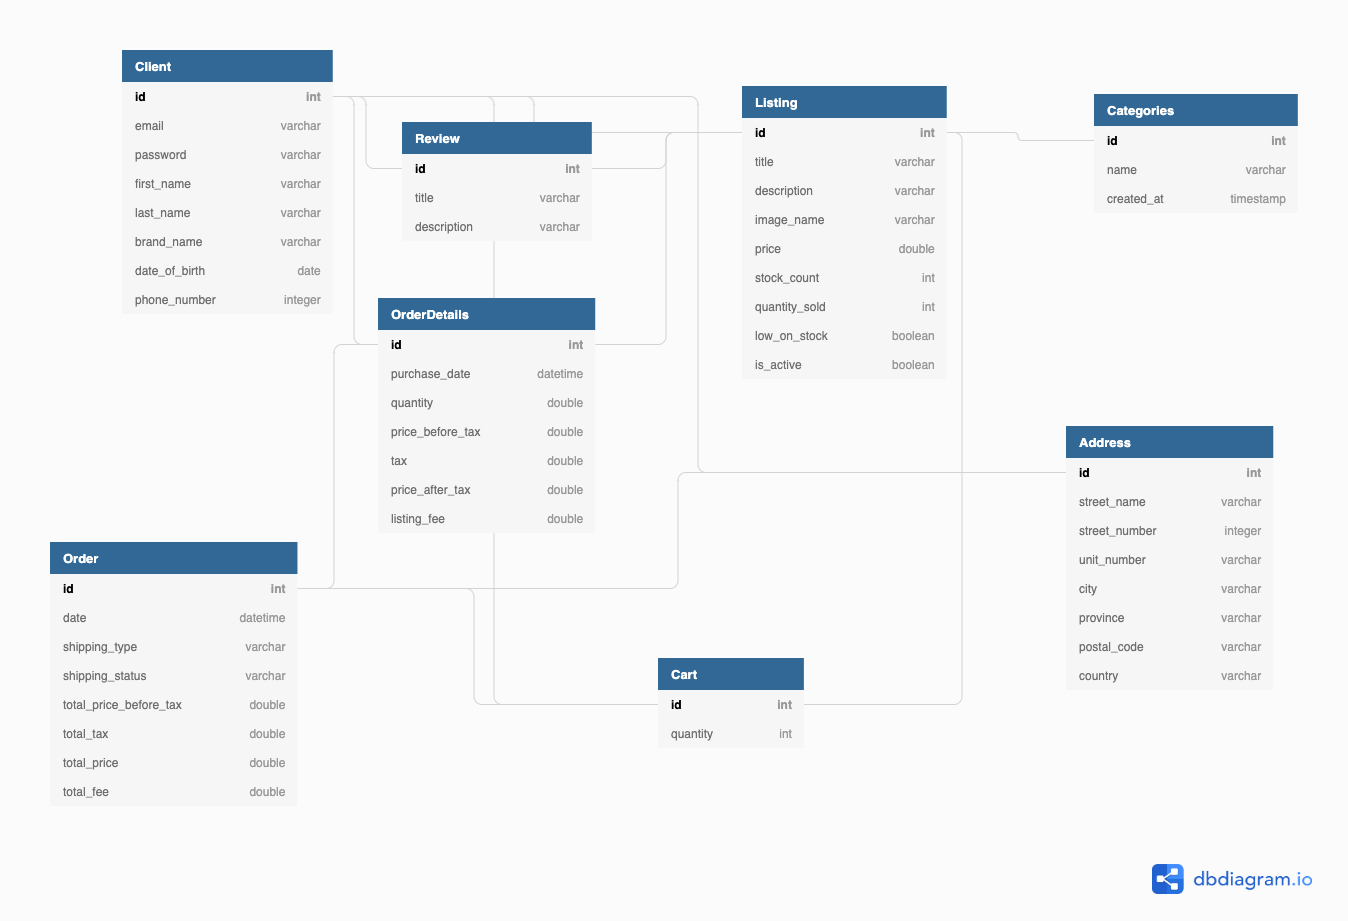
\includegraphics[width=0.9\textwidth]{Diagrams/ER/ER_Diagram_Typed.png}
    \caption{Database schemas}
    \label{fig:ER_Typed}
\end{figure}

\begin{figure}[ht!]
    \centering
    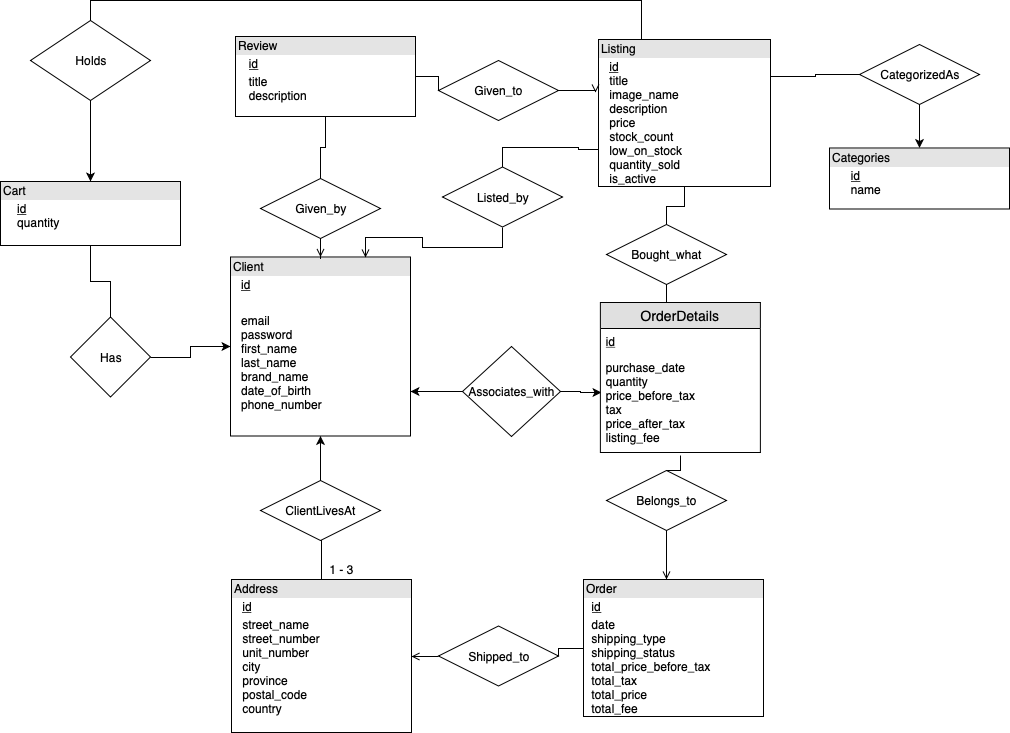
\includegraphics[width=0.9\textwidth]{Diagrams/ER/ER_Diagram.png}
    \caption{Entity Relationship Diagram}
    \label{fig:ER}
\end{figure}



\subsection{Description Of Each Entity}

\subsubsection{Client}
\textit{Client} is any user. They have the power to purchase and sell \textit{Listings}. A \textit{Client} can leave many \textit{Reviews}, create many \textit{Listings}, have many \textit{Carts}, and up to three \textit{Addresses}. Moreover, a \textit{Client} is associated with one \textit{OrderDetails} where the information related to their \textit{Orders} will be saved. Through referential integrity, \textit{Client}'s primary key consisting of its attribute \textit{id} is part of the primary key of \textit{Review} and \textit{Listing}. Finally, other attributes of \textit{Client} are \textit{email}, \textit{password}, \textit{first name}, \textit{last name}, \textit{brand name}, \textit{date of birth} and \textit{phone number}.

\subsubsection{Listings}
\textit{Listings} are the products sold and purchased on 354TheStars. Many \textit{Listings} are part of one \textit{Cart}, can have many \textit{Reviews}, and can be part of many \textit{OrderDetails}; however, a \textit{Listing} can only be listed by one \textit{Client} and can only have one \textit{Category}. Because of its relationship of referential integrity with \textit{Client}, \textit{Client}'s primary key will be part of that of \textit{Listing} in addition to \textit{Listing id}. Finally, the attributes belonging to \textit{Listing} are \textit{title}, \textit{image name}, \textit{description}, \textit{price}, \textit{stock count}, \textit{low on stock}, \textit{quantity sold}, and \textit{is active}.

\subsubsection{Address}
\textit{Address} contains information related to the shipping and/or billing place of preference of a \textit{Client}. Only one to three \textit{Addresses} are allowed per \textit{Client}, making the relationship between \textit{Address} and \textit{Client} many-to-one, respectively. Additionally, since an \textit{Order} is shipped to an address, \textit{Order} has referential integrity with \textit{Address}, making \textit{Address}'s primary key part of that of \textit{Order}.

\subsubsection{Order}
An \textit{Order} is shipped to an \textit{Address}, and the details of the order are stored in \textit{OrderDetails}. An \textit{Order} cannot exist without an \textit{Address} due to referential integrity; therefore \textit{Address}'s primary key will be part of that of \textit{Order}. Similarly, because of referential integrity \textit{Order}'s primary key will also be part of \textit{OrderDetails}. This means the primary key of \textit{Order} is composed by \textit{Address id} and \textit{Order id}. \textit{Order} also counts with the attributes \textit{date}, \textit{shipping type}, \textit{shipping status}, \textit{total price before tax}, \textit{total tax}, \textit{total price} and \textit{total fee}.

\subsubsection{Review}
A \textit{Review} is an assessment a \textit{Client} leaves on a \textit{Listing} following a sale. Only those \textit{Buyers} who purchased said \textit{Listing} are allowed to write reviews for that specific \textit{Listing}. Given this, a \textit{Review} can not exist neither without a \textit{Client} acting as the author, nor without a \textit{Listing} to receive said \textit{Review}, leading to referential integrity of type many-to-many with both the \textit{Client} and the \textit{Listing}. Moreover, with referential integrity, a \textit{Review} has an \textit{id}, and two foreign keys: the \textit{id} of the \textit{Client} who creates a \textit{Review}, and the primary key of the \textit{Listing} who receives the \textit{Review}. These three keys act as the primary key of \textit{Review}. Aside from this, \textit{Review} has a title and a description. Finally, an \textit{Address} has an \textit{id} as primary key, and other attributes such as \textit{street name}, \textit{street number}, \textit{unit number}, \textit{city}, \textit{province}, \textit{postal code} and \textit{country}.

\subsubsection{Order Details}
\textit{OrderDetails} contains information related to an \textit{Order} and what \textit{Listings} were bought with it. Its attributes are \textit{id}, which is the primary key, and \textit{purchase date}, \textit{quantity}, \textit{price before tax}, \textit{tax}, \textit{price price after tax} and \textit{listing fee}. Many \textit{Listings} can be in many \textit{OrderDetails}, yet there can only be one \textit{OrderDetails} per \textit{Order}; therefore, because of referential integrity, the \textit{OrderDetails} has \textit{Order id} as a foreign key, and part of its primary key. Finally, \textit{OrderDetails} is associated with the \textit{Client} who placed the \textit{Order}.

\subsubsection{Category}
\textit{Category} offers a classification system for \textit{Listing}. It has an \textit{id} as primary key, and an attribute \textit{name} that describes what the \textit{Category} represents. All categories can belong to many \textit{Listings}.

\subsubsection{Cart}
\textit{Cart} is related to \textit{Listing} and \textit{Client}. Many \textit{Listings} belong to one \textit{Cart} in which the \textit{quantity} ordered of that \textit{Listing} is stored. Likewise, many \textit{Carts} can belong to one \textit{Client}. The primary key of \textit{Cart} is its \textit{id}.
\clearpage

\section{Class Diagram}
\begin{figure}[ht!]
    \centering
    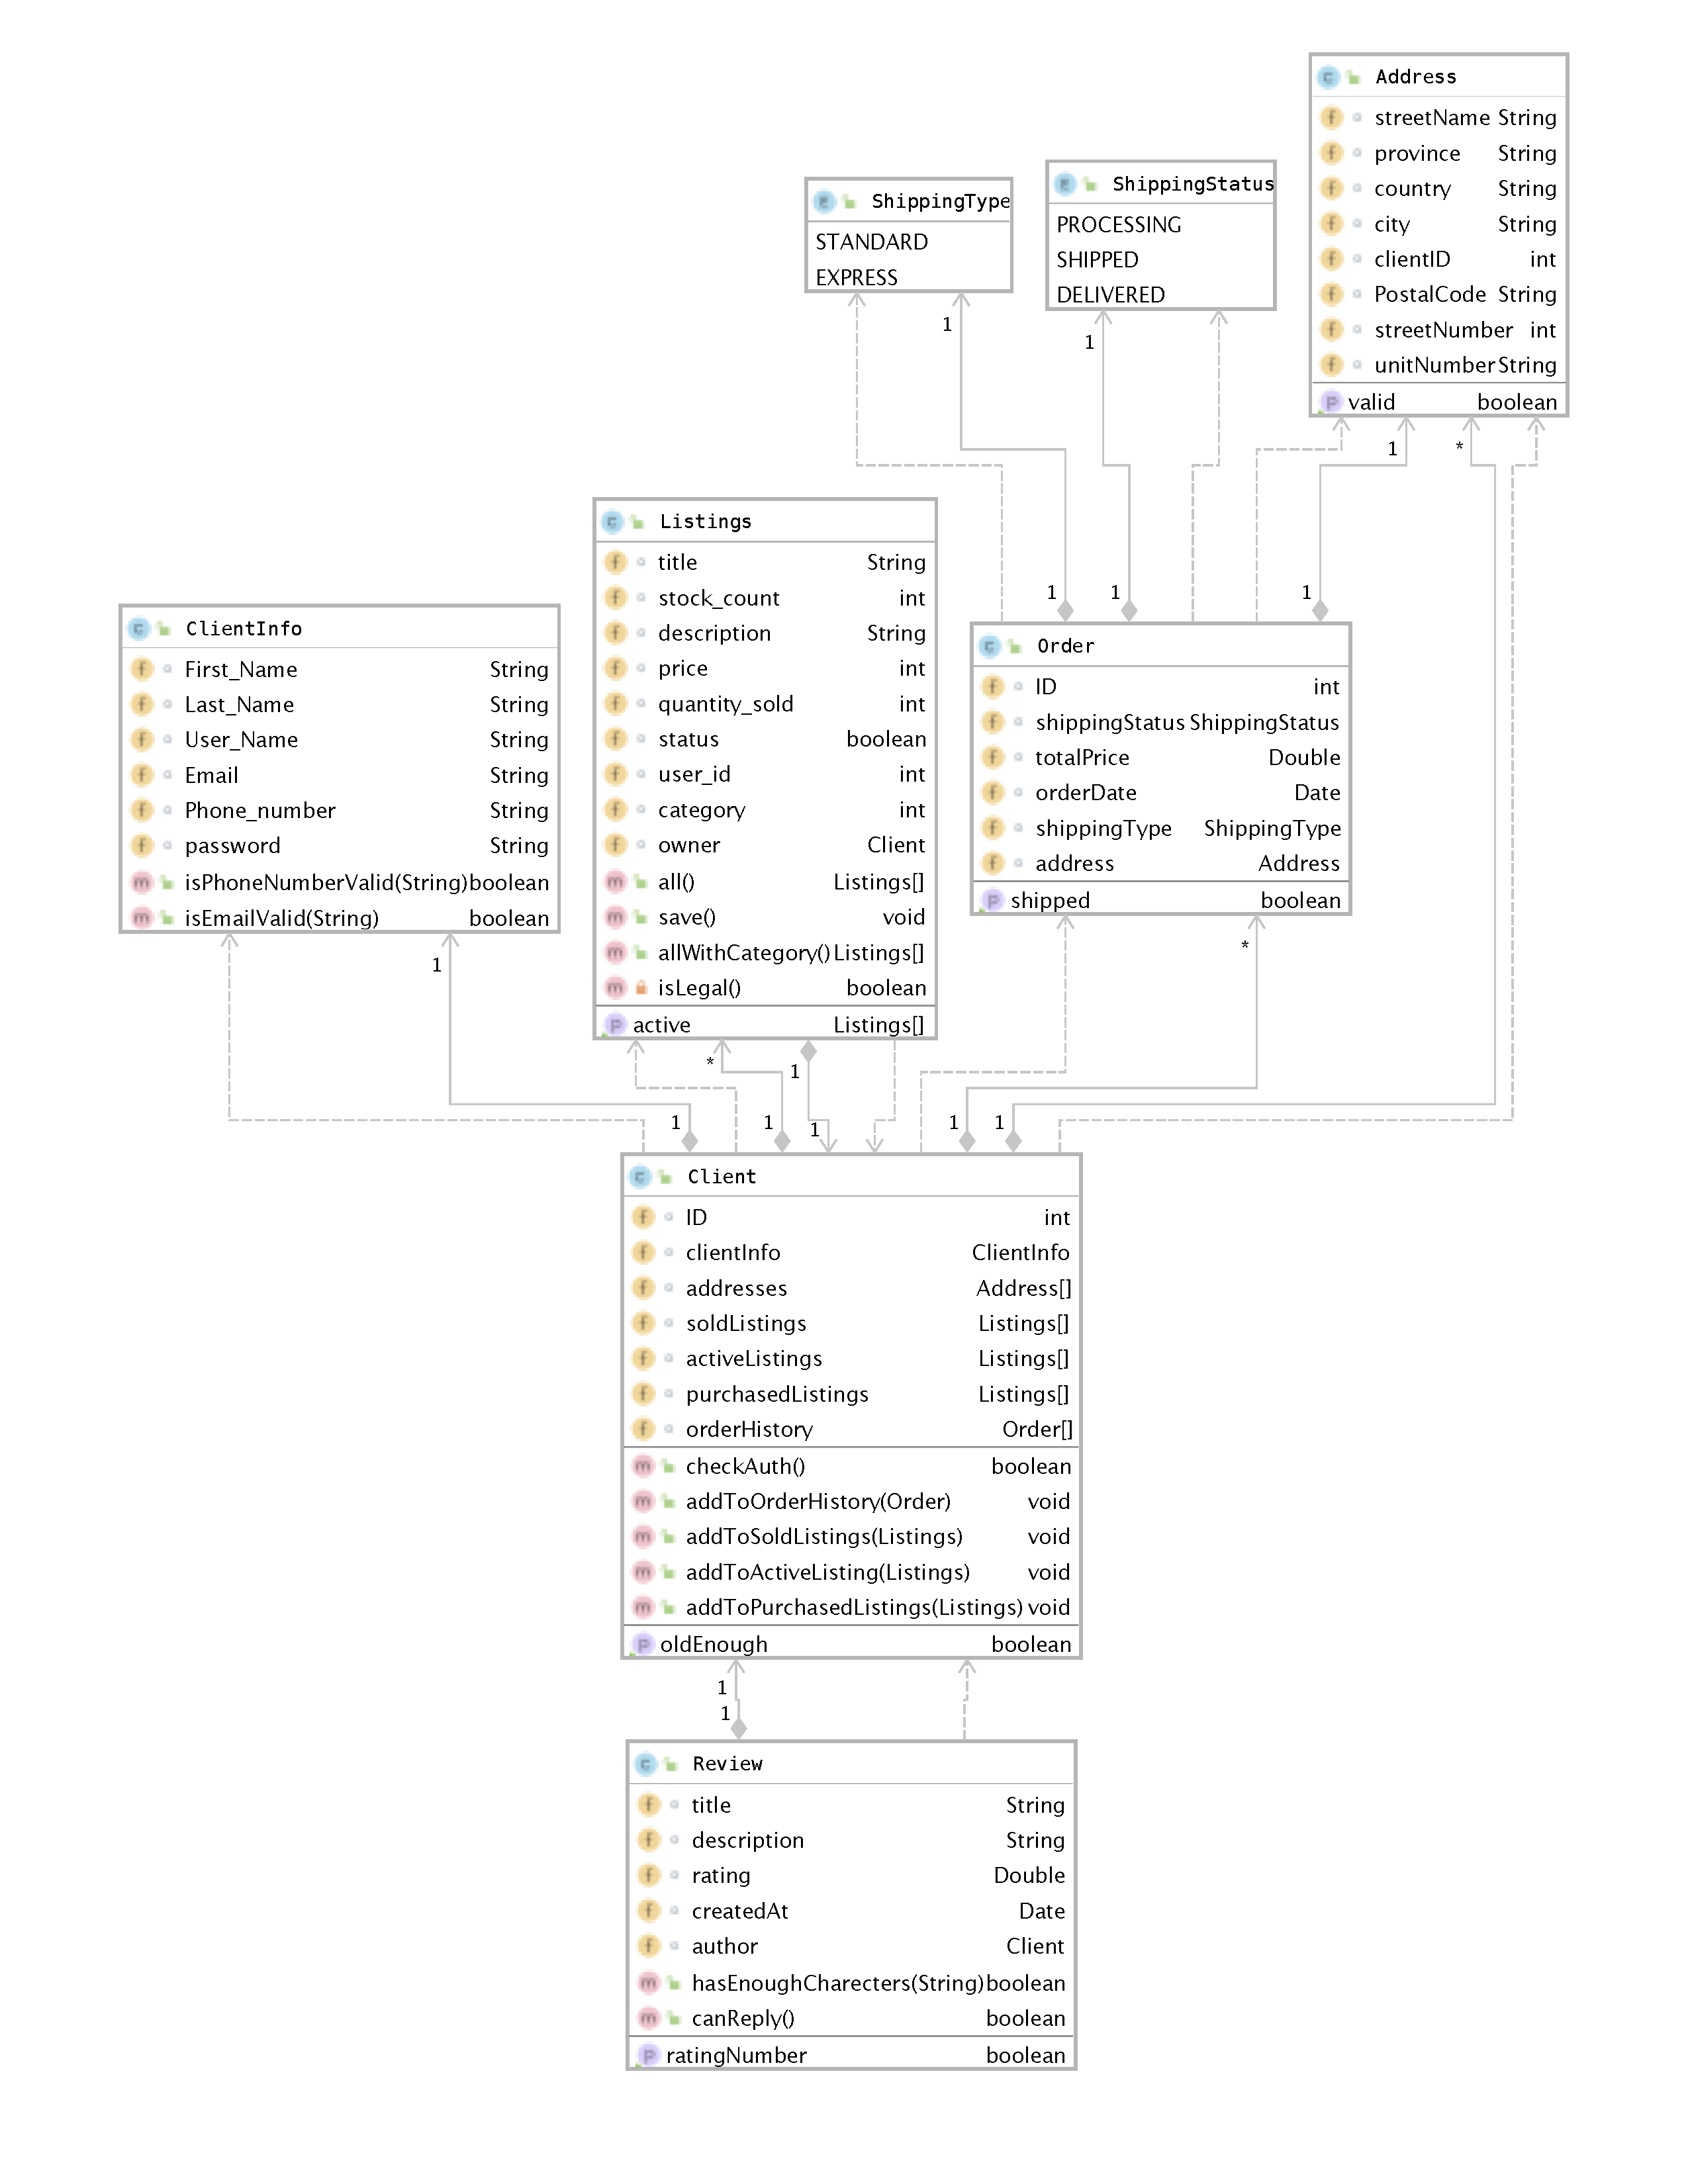
\includegraphics[width=0.8\textwidth]{Diagrams/Class/class_diagram.png}
    \caption{Class Diagram}
    \label{fig: Class diagram}
\end{figure}

\subsection{Description Of Class Diagram}
\subsubsection{Client}
\textit{Client} is any user. They have the power to purchase and sell \textit{Listings}. A \textit{Client} can leave many \textit{Reviews}, create many \textit{Listings}, and up to three \textit{Addresses}. Moreover, a \textit{Client} is associated with \textit{Orders}. Through referential integrity, \textit{Client}'s primary key consisting of its attribute \textit{id} is part of the primary key of \textit{Review} and \textit{Listing}. Finally, other attributes of \textit{Client} are \textit{email}, \textit{password}, \textit{first name}, \textit{last name}, \textit{brand name}, \textit{date of birth} and \textit{phone number}.

\subsubsection{ClientInfo}
\textit{ClientInfo} is all the personal infromation about a client. ClientInfo class consists of \textit{email}, \textit{password}, \textit{first name}, \textit{last name}, \textit{brand name}, \textit{date of birth} and \textit{phone number}.

\subsubsection{Listings}
\textit{Listings} are the products sold and purchased on 354TheStars. Many \textit{Listings} can have many \textit{Reviews}, however, a \textit{Listing} can only be listed by one \textit{Client}. Because of its relationship of referential integrity with \textit{Client}, \textit{Client}'s primary key will be part of that of \textit{Listing} in addition to \textit{Listing id}. Finally, the attributes belonging to \textit{Listing} are \textit{title}, \textit{image name}, \textit{description}, \textit{price}, \textit{stock count}, \textit{low on stock}, \textit{quantity sold}, and \textit{is active}.

\subsubsection{Address}
\textit{Address} contains information related to the shipping and/or billing place of preference of a \textit{Client}. Only one to three \textit{Addresses} are allowed per \textit{Client}, making the relationship between \textit{Address} and \textit{Client} many-to-one, respectively. Additionally, since an \textit{Order} is shipped to an address, \textit{Order} has referential integrity with \textit{Address}, making \textit{Address}'s primary key part of that of \textit{Order}.

\subsubsection{Order}
An \textit{Order} is shipped to an \textit{Address}. An \textit{Order} cannot exist without an \textit{Address} due to referential integrity; therefore \textit{Address}'s primary key will be part of that of \textit{Order}. This means the primary key of \textit{Order} is composed by \textit{Address id}. \textit{Order} also counts with the attributes \textit{date}, \textit{shipping type}, \textit{shipping status}, \textit{total price before tax}, \textit{total tax}, \textit{total price} and \textit{total fee}.

\subsubsection{Review}
A \textit{Review} is an assessment a \textit{Client} leaves on a \textit{Listing} following a sale. Only those \textit{Buyers} who purchased said \textit{Listing} are allowed to write reviews for that specific \textit{Listing}. Given this, a \textit{Review} can not exist neither without a \textit{Client} acting as the author, nor without a \textit{Listing} to receive said \textit{Review}, leading to referential integrity of type many-to-many with both the \textit{Client} and the \textit{Listing}. Moreover, with referential integrity, a \textit{Review} has an \textit{id}, and two foreign keys: the \textit{id} of the \textit{Client} who creates a \textit{Review}, and the primary key of the \textit{Listing} who receives the \textit{Review}. These three keys act as the primary key of \textit{Review}. Aside from this, \textit{Review} has a title and a description. Finally, an \textit{Address} has an \textit{id} as primary key, and other attributes such as \textit{street name}, \textit{street number}, \textit{unit number}, \textit{city}, \textit{province}, \textit{postal code} and \textit{country}.





\section{Sequence Diagrams}

\begin{figure}[ht!]
    \subsection{Add Review to Listing}
    \centering
    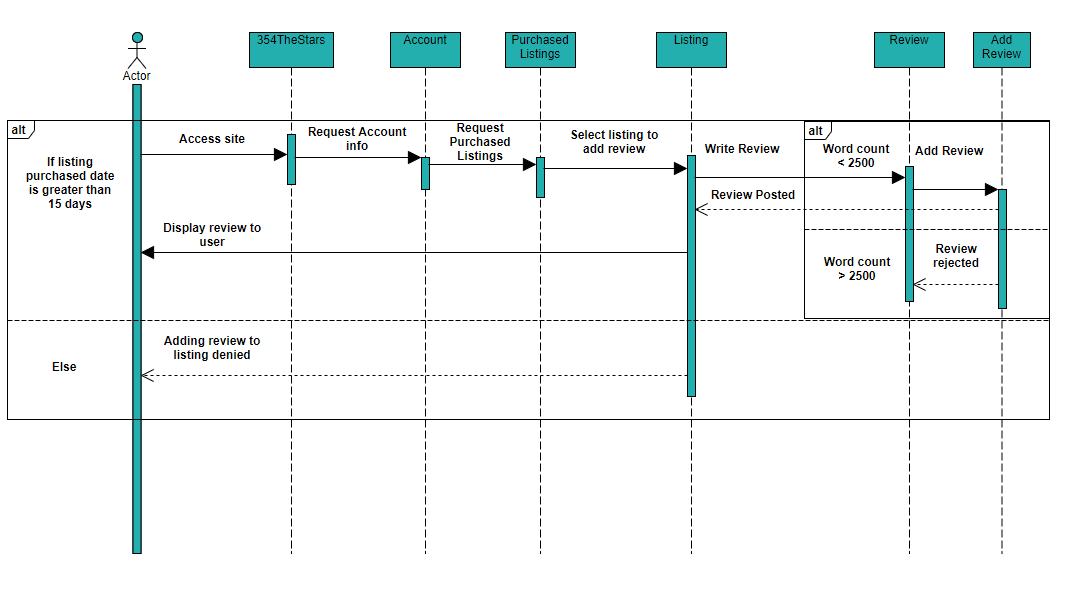
\includegraphics[width=0.8\textwidth,height=0.3\paperheight]{Diagrams/Sequence/Add_Review.png}
    \caption{Sequence Diagram 1: Add Review to Listing}
    \label{fig: Add Review to Listing}
    \begin{justify}
        The add review sequence diagram shows the steps the user
        needs to take to add a review to an item. The user will access their account, go to the purchased listings section and if the purchased date is greater than 15 days, it will allow the user to add a review, otherwise it will not. Once the item has been selected, user will write the review. If the character count is less than or equal to 400, the review will be submitted, else it will be rejected.
    \end{justify}
\end{figure}

\begin{figure}[ht!]
    \subsection{Cart Operations}
    \centering
    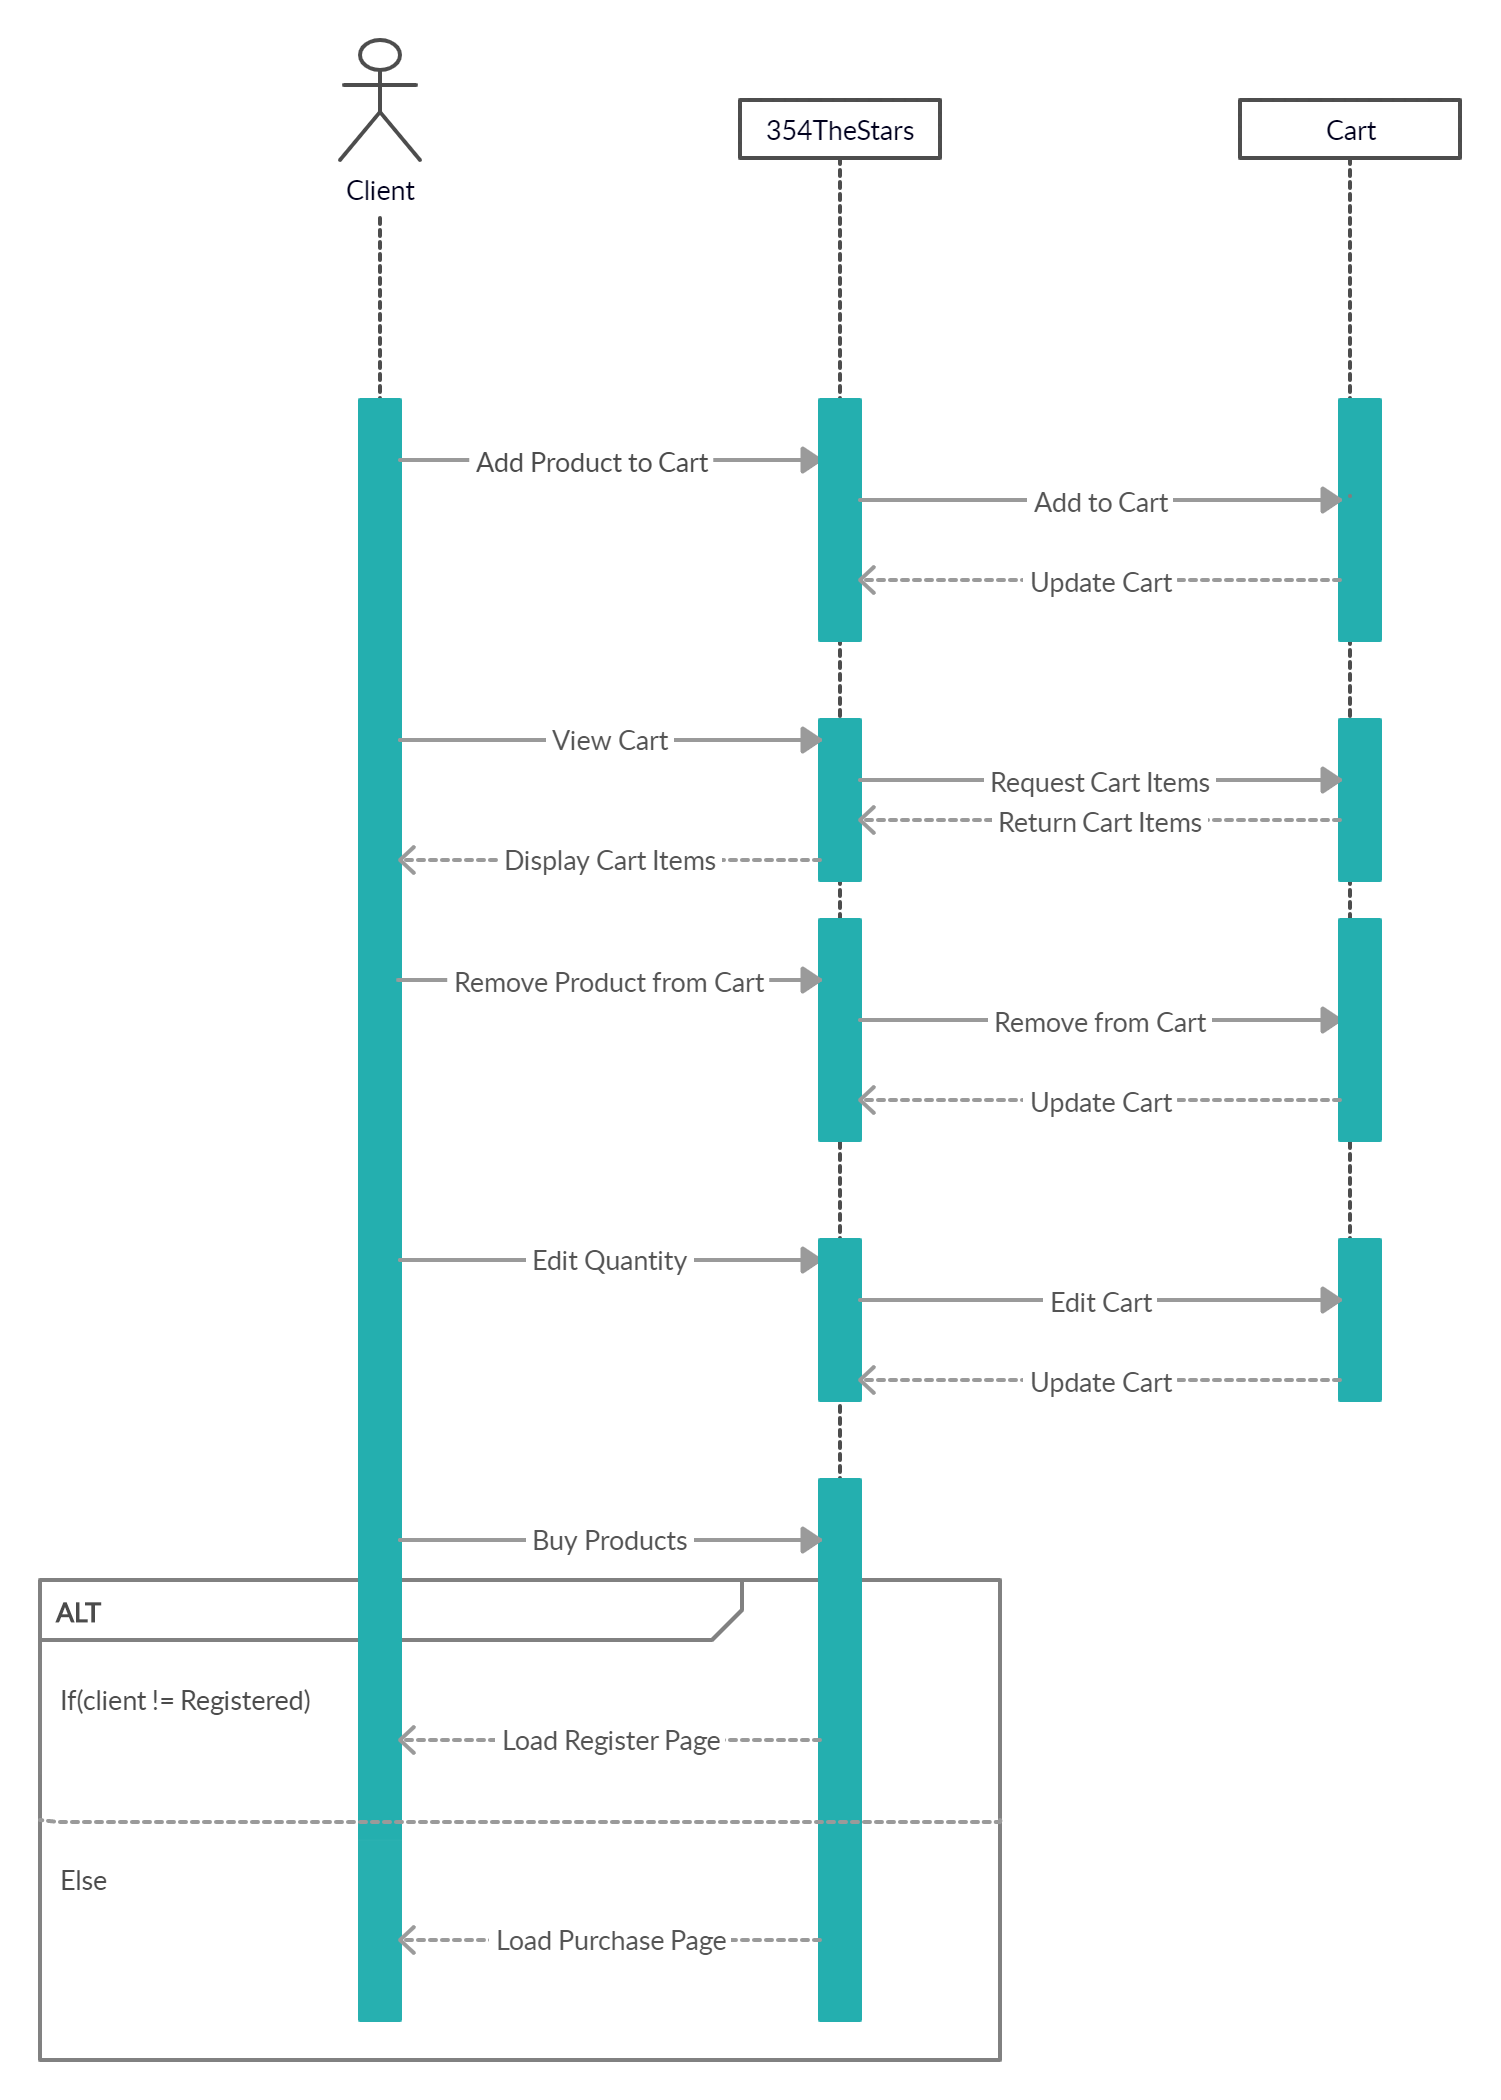
\includegraphics[width=0.65\textwidth,height=0.45\paperheight]{Diagrams/Sequence/Cart_Operations.jpg}
    \caption{Sequence Diagram 2: Cart Operations}
    \label{fig: Cart Operations}
    \begin{justify}
        A product can be added to cart when the client clicks on "Add Product to Cart". A client can also choose to view items in their cart. When the items from their cart are displayed, the client can choose to either remove a product from the cart or edit quantity of an item in the cart. The cart will be updated after those actions are performed. When the client clicks on "Buy Products", if the client is a guest user, they will be redirected into the registration page. Otherwise, if the client is a registered user, the purchase page will be loaded.
    \end{justify}
\end{figure}

\begin{figure}[ht!]
    \subsection{Checkout}
    \centering
    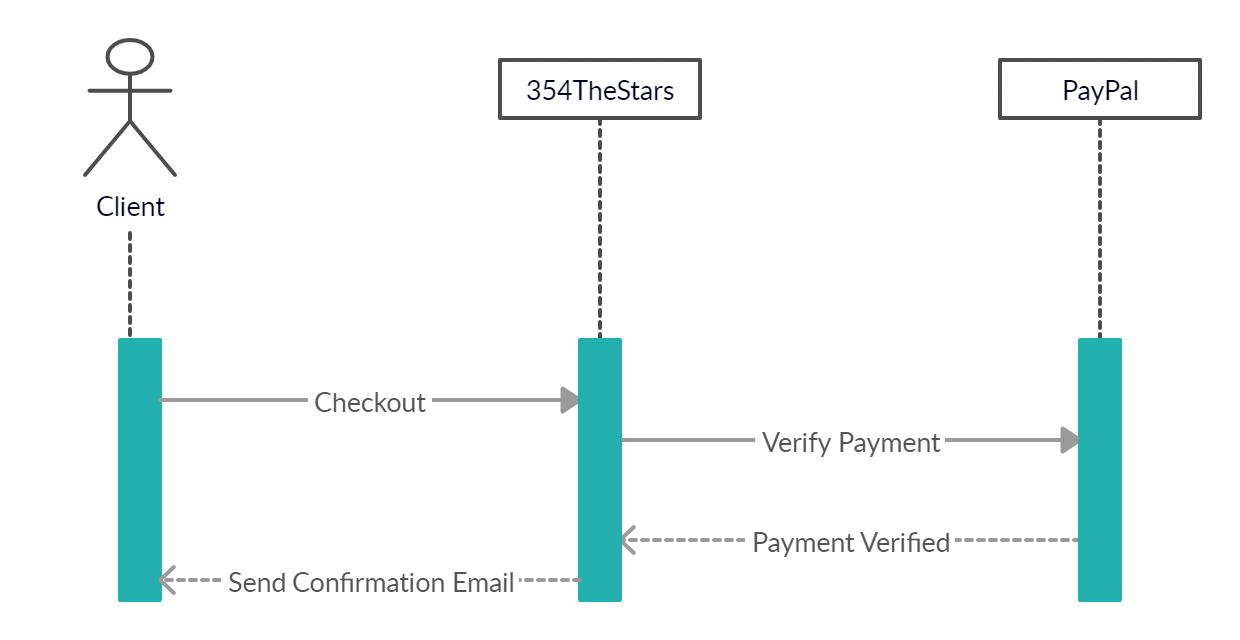
\includegraphics[width=0.6\textwidth,height=0.15\paperheight]{Diagrams/Sequence/Checkout.jpg}
    \caption{Sequence Diagram 3: Checkout}
    \label{fig: Checkout}
    \begin{justify}
        When the client clicks on checkout, the system will automatically verify the payment with PayPal. As soon as the payment is verified, a confirmation email will be sent to the client.
    \end{justify}
\end{figure}

\begin{figure}[ht!]
    \subsection{Edit Client Information}
    \centering
    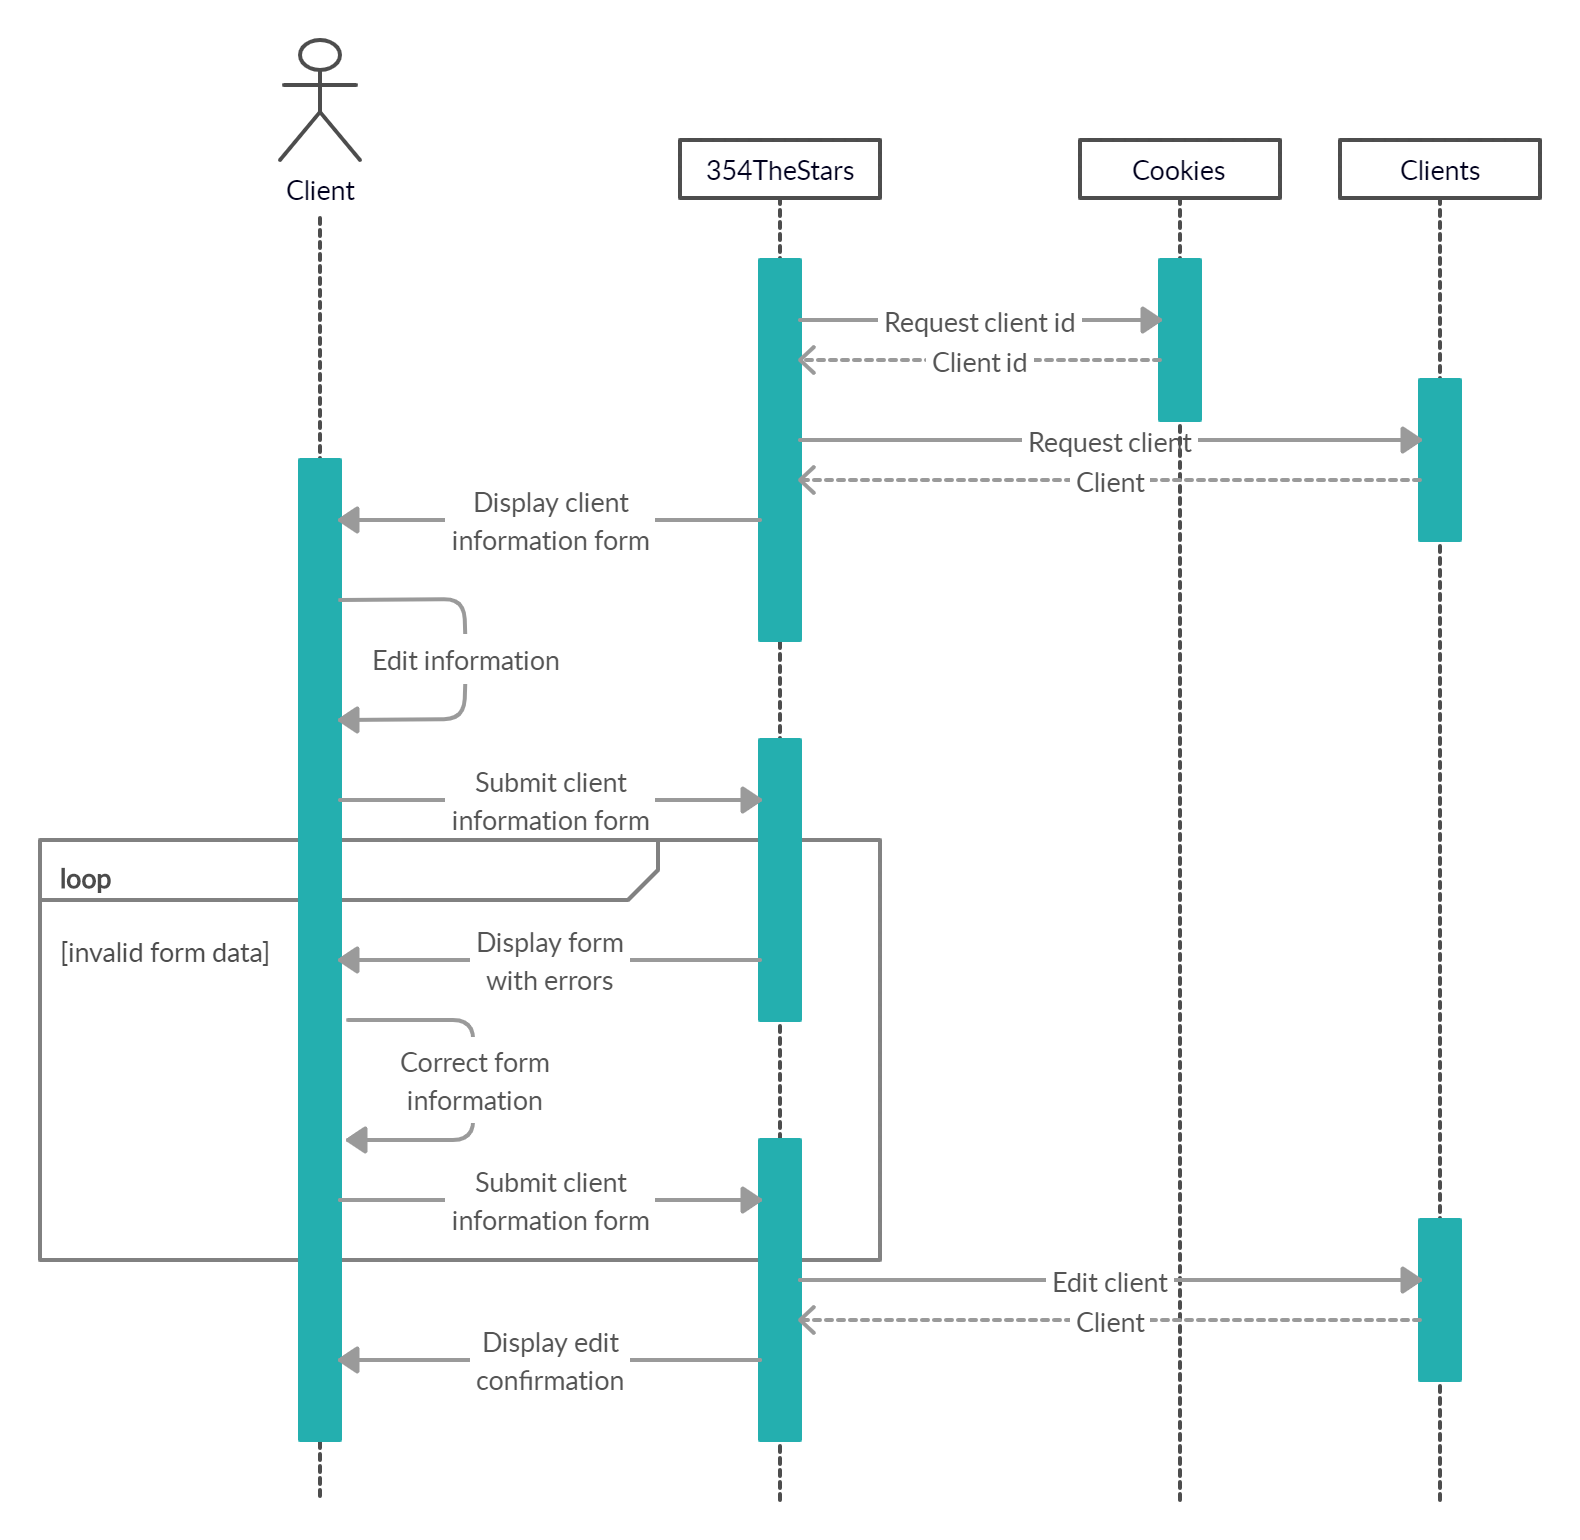
\includegraphics[width=0.65\textwidth,height=0.3\paperheight]{Diagrams/Sequence/Edit_Client_Info.jpg}
    \caption{Sequence Diagram 4: Edit Client Information}
    \label{fig: Edit Client Information}
    \begin{justify}
        First, the website retrieves the client’s ID through cookies which is then used to query the Clients table in the database. With this, the client’s information is retrieved from the database and displayed to the client through an editable form. Next, the client edits the information in this form and submits it. If this form contains invalid data, the website re-displays the form, indicating the invalid data. The client then corrects the form and resubmits it, which is then validated once again and so, until the data in the form is valid. Finally, the website edits the corresponding client entity in the Client table of the database and the database returns the edited client. This ends with a confirmation displayed to the client indicating that the edit was successful.
    \end{justify}
\end{figure}

\begin{figure}[ht!]
    \subsection{Filter Listings Results}
    \centering
    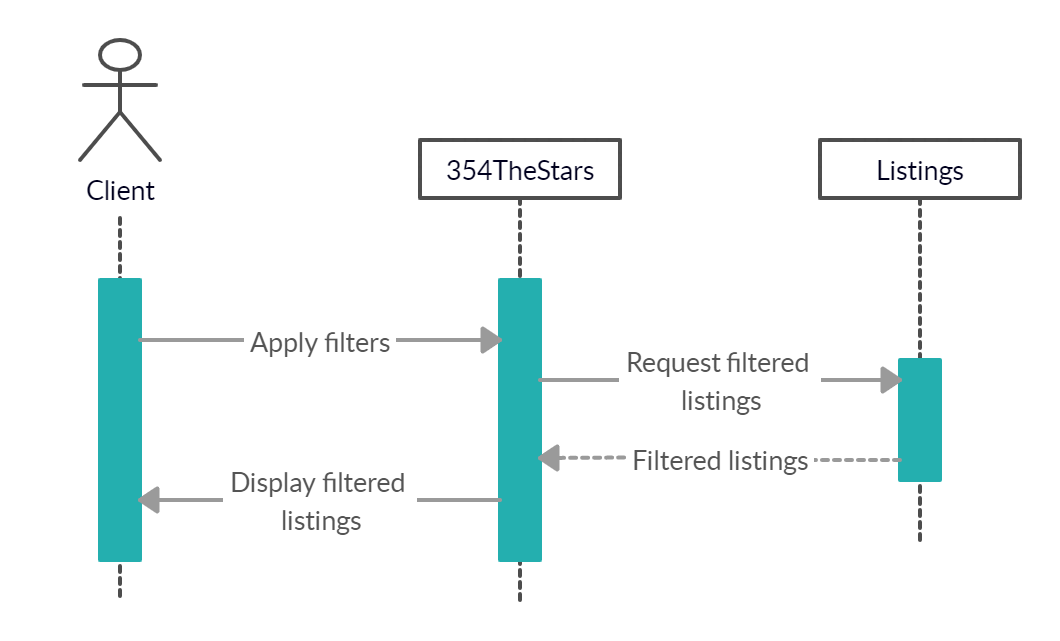
\includegraphics[width=0.5\textwidth,height=0.15\paperheight]{Diagrams/Sequence/Filter_Listings.jpg}
    \caption{Sequence Diagram 5: Filter Listings Results}
    \label{fig: Filter Listings Results}
    \begin{justify}
        The client starts by applying filters to the list of listings. The website then takes these filter parameters and uses them to query the Listings table in the database. The filtered listings is then retrieved from the database and displayed to the client.
    \end{justify}
\end{figure}

\begin{figure}[ht!]
    \subsection{Get Listings Details}
    \centering
    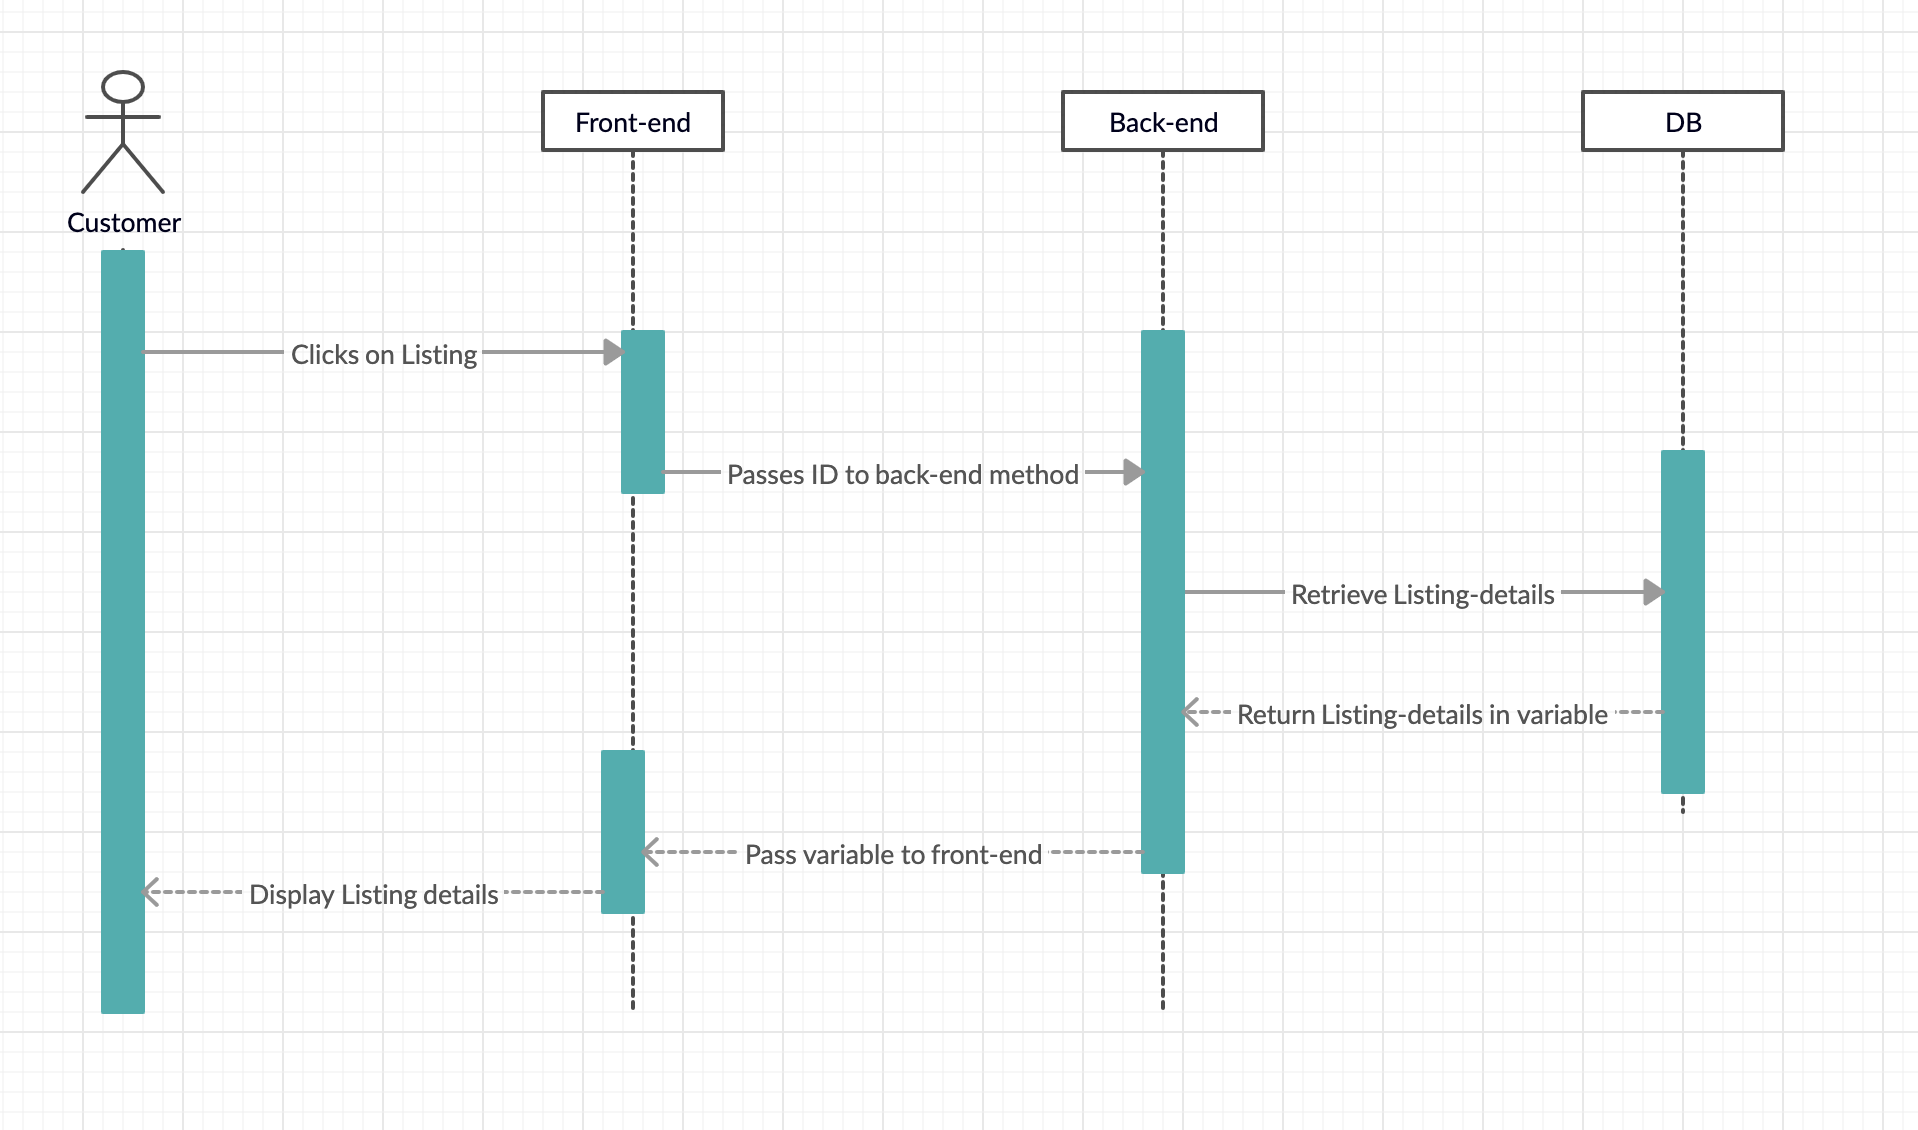
\includegraphics[width=0.7\textwidth,height=0.25\paperheight]{Diagrams/Sequence/Listing_Details.png}
    \caption{Sequence Diagram 6: Get Listing Details}
    \label{fig: Get Listing Details}
    \begin{justify}
        This diagram represents the process of retrieving the details for each listing. In other words, the process that is going to take place when a customer clicks on a listing. Clicking on the listing will call a method from the backend by passing the listing ID to it. After which, the method retrieves the listing details, and stores them in a variable. That variable is then called by the front end, which in turn, displays the listing details on screen for the customer.
    \end{justify}
\end{figure}

\begin{figure}[ht!]
    \subsection{Get Lists of Listings}
    \centering
    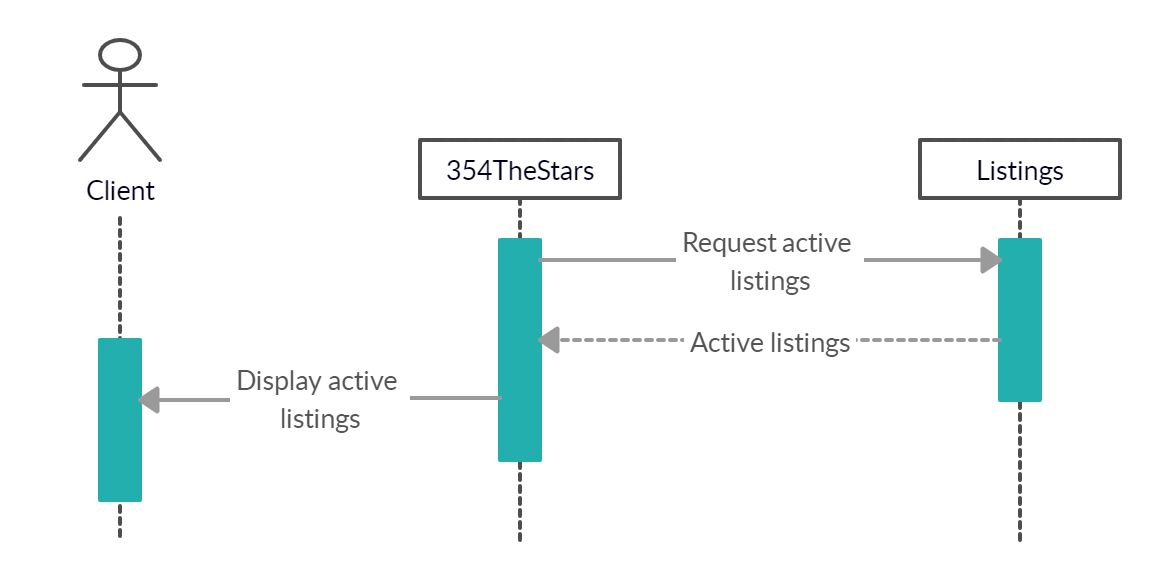
\includegraphics[width=0.5\textwidth,height=0.15\paperheight]{Diagrams/Sequence/Lists_of_Listings.jpg}
    \caption{Sequence Diagram 7: Get Lists Of Listings}
    \label{fig: Get Lists Of Listings}
    \begin{justify}
        The website queries the Listings table in the database for listings which have the status field set to true. The active listings are then retrieved from the database and displayed to the client.
    \end{justify}
\end{figure}

\begin{figure}[ht!]
    \subsection{Get Order History}
    \centering
    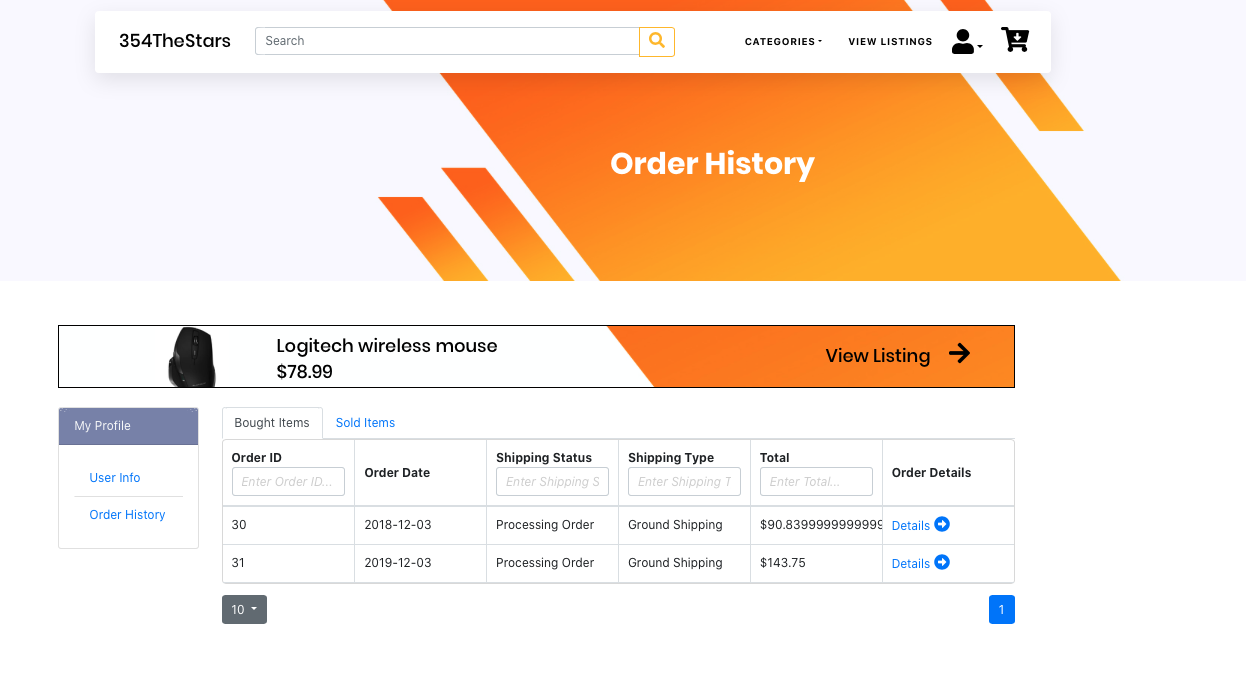
\includegraphics[width=0.65\textwidth,height=0.2\paperheight]{Diagrams/Sequence/Order_History.png}
    \caption{Sequence Diagram 8: Get Order History}
    \label{fig: Get Order History}
    \begin{justify}
       The order history sequence diagram shows the steps the user needs to take to view their order history. User has to access their account and if the number of purchased item is 0 then it will display no history. Otherwise it will display the history of all the purchased items from the user.
    \end{justify}
\end{figure}

\begin{figure}[ht!]
    \subsection{Login}
    \centering
    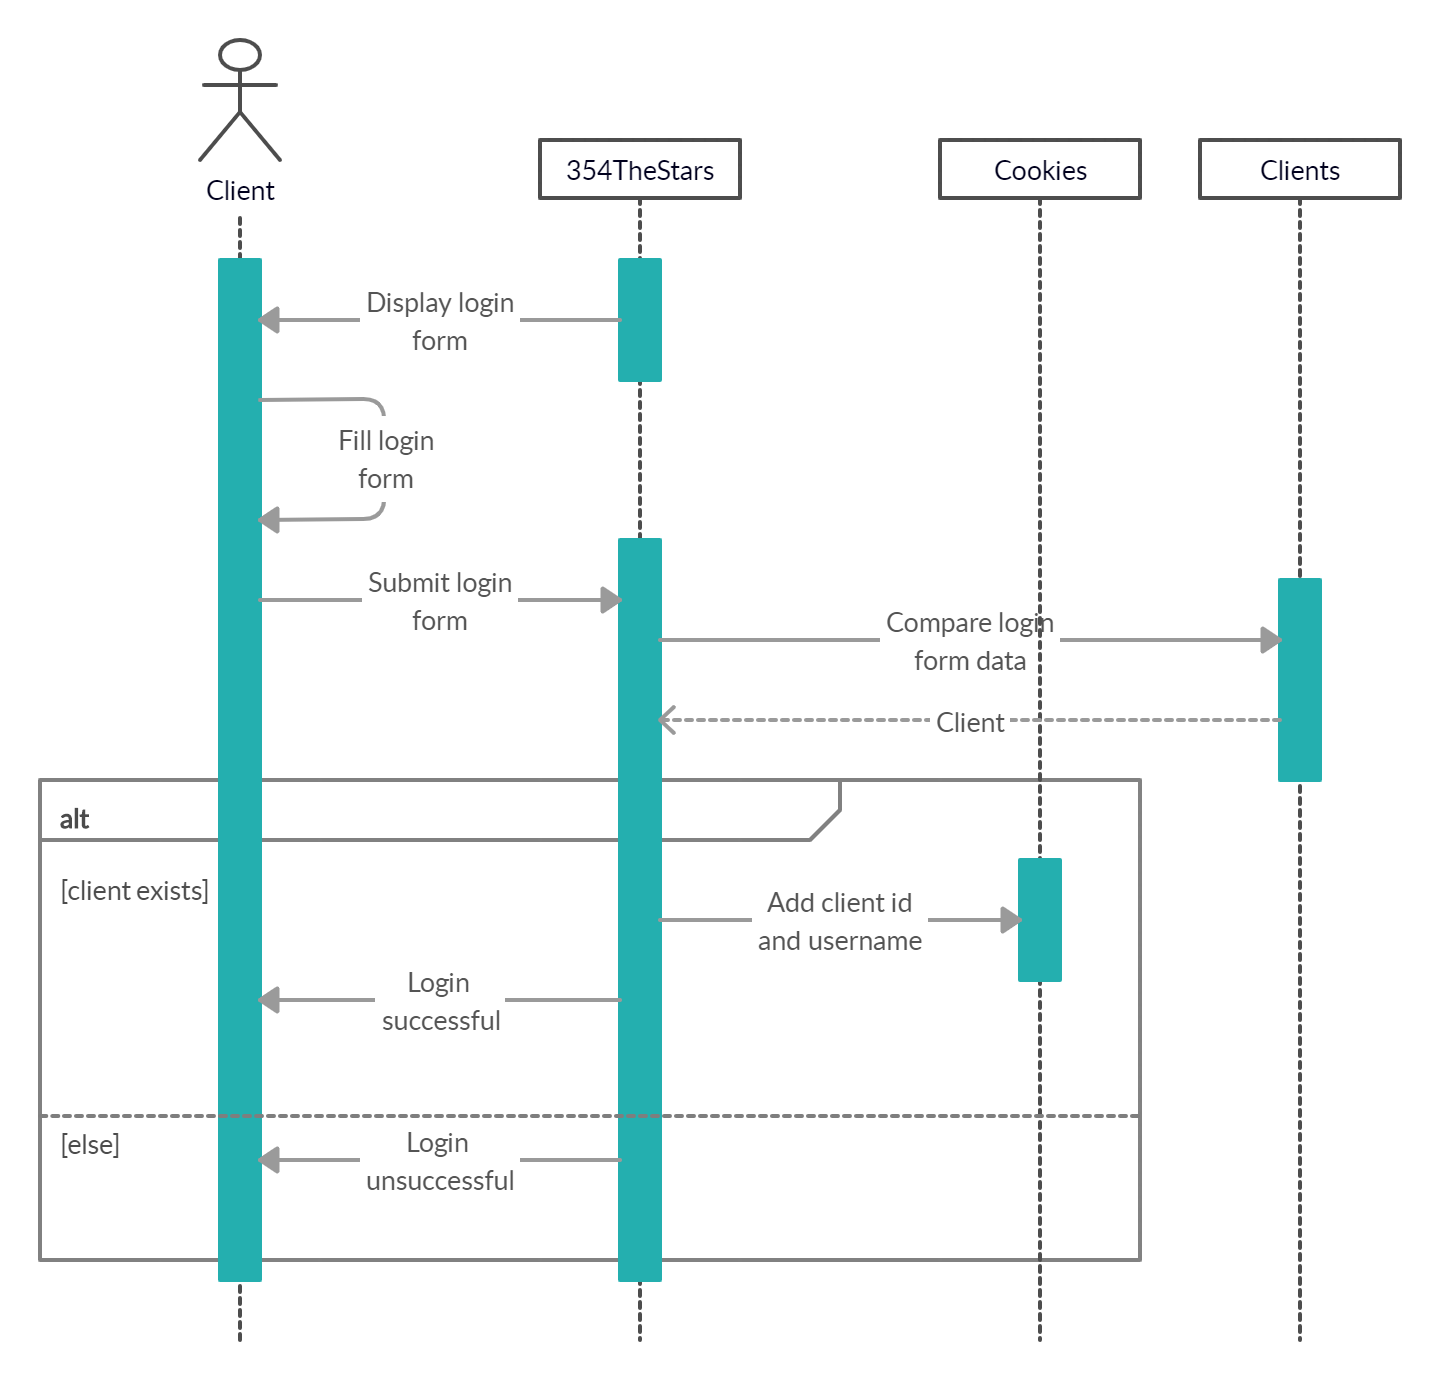
\includegraphics[width=0.6\textwidth,height=0.3\paperheight]{Diagrams/Sequence/Login.jpg}
    \caption{Sequence Diagram 9: Login}
    \label{fig: Login}
    \begin{justify}
        The website displays a login form to the client who fills it and submits it. The form data is used to query the Client table in the database. Of course, since passwords are encrypted before stored, some manipulation to the password form data needs to be performed beforehand. If a client entity is retrieved from the database, then the client’s id and client's name is stored in cookies and the client is notified that the login was successful. Otherwise, an error message is displayed informing the client that the login was unsuccessful.
    \end{justify}
\end{figure}

\begin{figure}[ht!]
    \subsection{Logout}
    \centering
    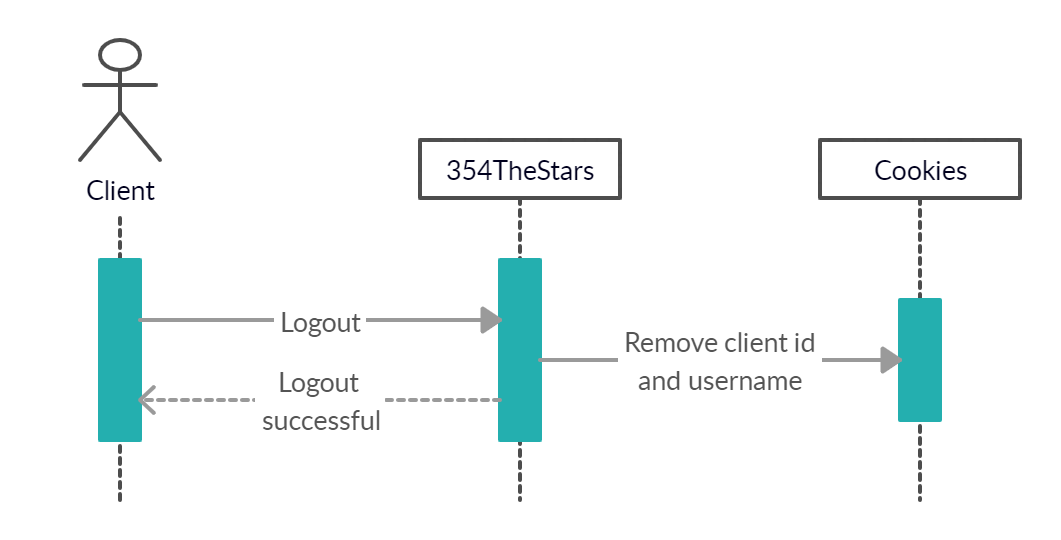
\includegraphics[width=0.5\textwidth,height=0.15\paperheight]{Diagrams/Sequence/Logout.jpg}
    \caption{Sequence Diagram 10: Logout}
    \label{fig: Logout}
    \begin{justify}
        When the client clicks the logout button, the website removes the client’s id and client's name from cookies and indicates to the client that the logout was successful.
    \end{justify}
\end{figure}

\begin{figure}[ht!]
    \subsection{Register}
    \centering
    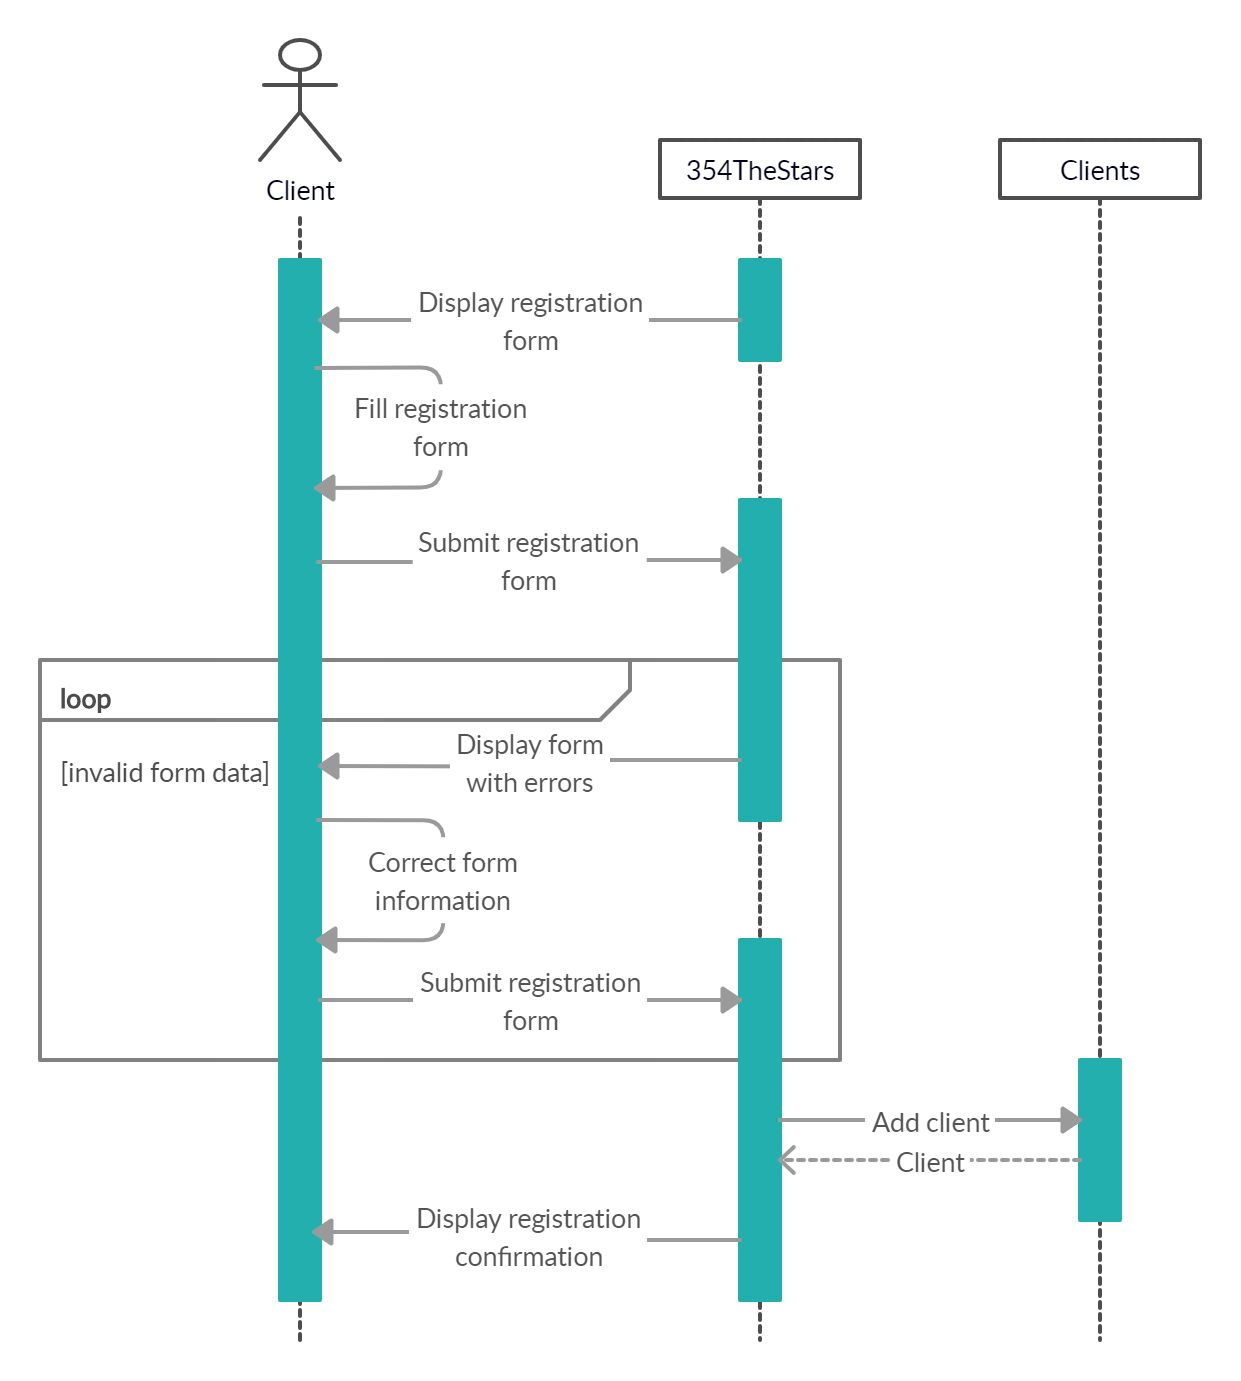
\includegraphics[width=0.6\textwidth,height=0.3\paperheight]{Diagrams/Sequence/Register.jpg}
    \caption{Sequence Diagram 11: Register}
    \label{fig: Register}
    \begin{justify}
        The website displays a registration form to the client who fills it and submits it. While the form has invalid data, the website re-displays this form to the client, indicating the invalid data. The client then proceeds to correct the form and resubmit it for validation. When the form is valid, the website adds a client to the Clients table in the database and returns the newly added client. This process ends with a confirmation displayed to the client indicating that the registration was successful.
    \end{justify}
\end{figure}

\begin{figure}[ht!]
    \subsection{Purchase by a Registered User}
    \centering
    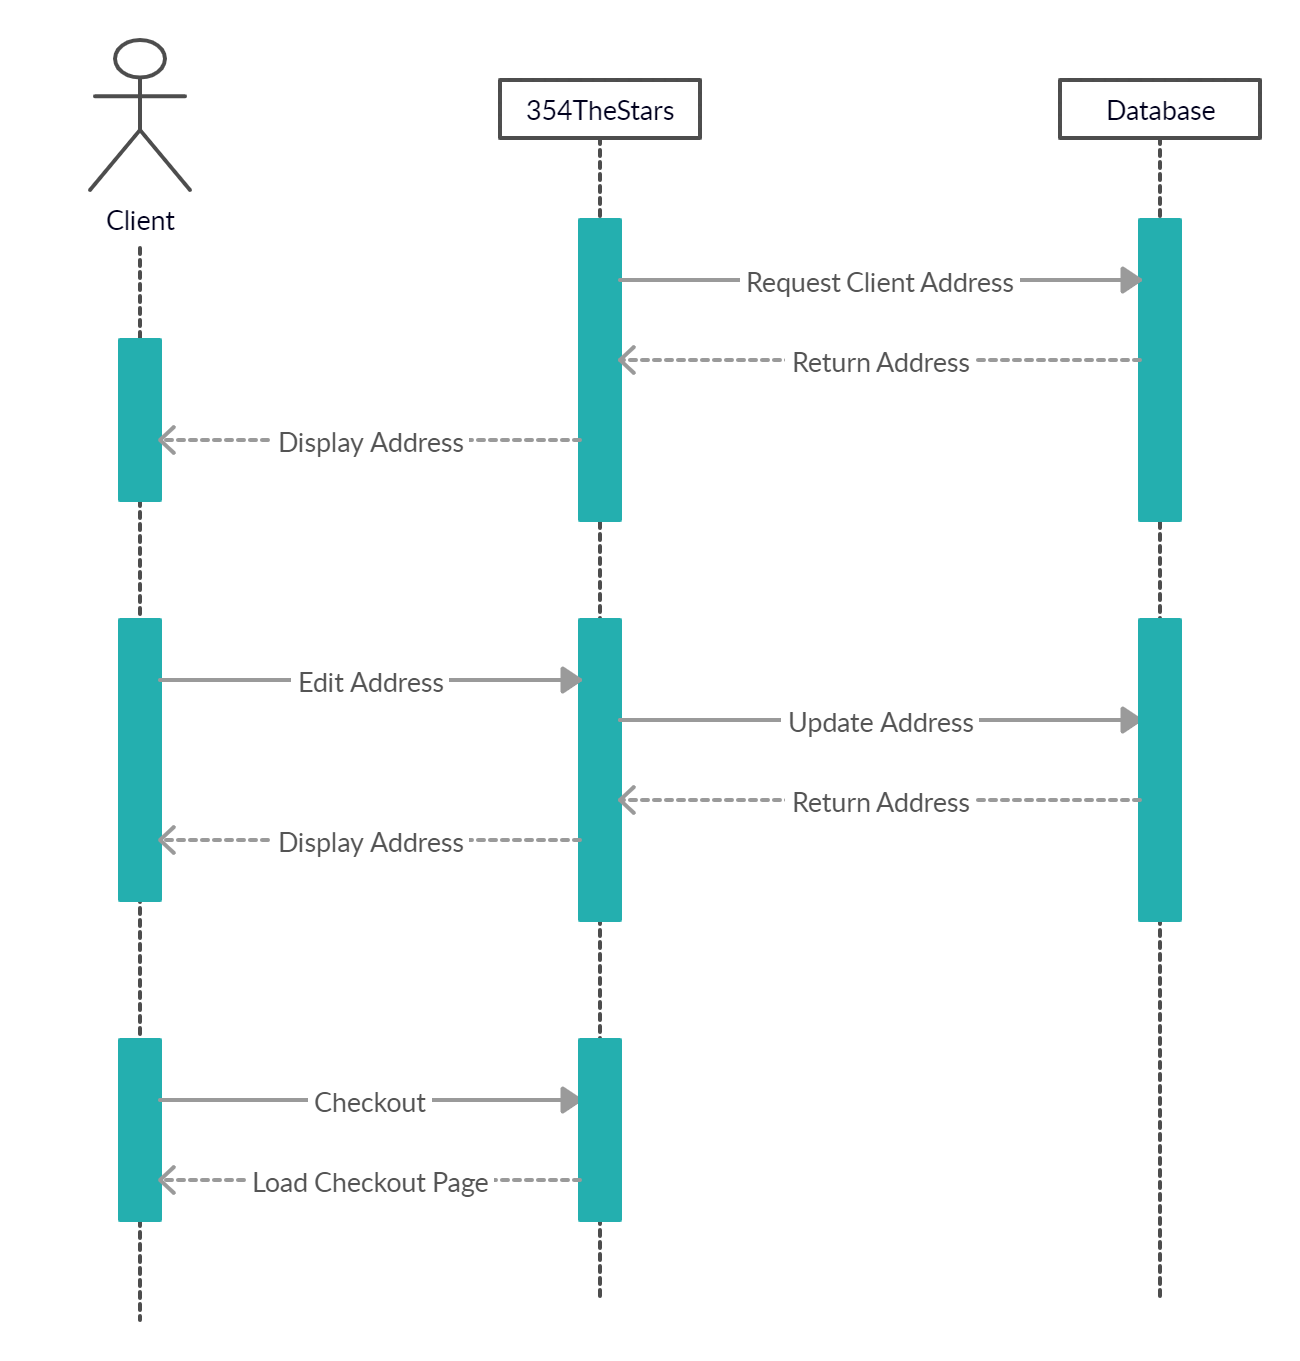
\includegraphics[width=0.6\textwidth,height=0.3\paperheight]{Diagrams/Sequence/Registered_User_Purchase.jpg}
    \caption{Sequence Diagram 12: Purchase by a Registered User}
    \label{fig: Purchase by a Registered User}
    \begin{justify}
        When the purchase page is loaded, the client's address will be displayed. The client can edit the address and the database will update and will display the new address. When the user clicks on checkout, the website will redirect the user in the checkout page.
    \end{justify}
\end{figure}

\begin{figure}[ht!]
    \subsection{Select Listing Category}
    \centering
    \includegraphics[width=0.65\textwidth,height=0.2\paperheight]{Diagrams/Sequence/Categories.png}
    \caption{Sequence Diagram 13: Select Listing Category}
    \label{fig: Select Listing Category}
    \begin{justify}
        The categories sequence diagram shows the steps the user needs to take to access the different categories on the website. On the page, the user will select the categories tab and select the specific category to display. The requested listing will then be shown to the user.
    \end{justify}
\end{figure}

\begin{figure}[ht!]
    \subsection{Send Confirmation Email}
    \centering
    \includegraphics[width=0.6\textwidth,height=0.15\paperheight]{Diagrams/Sequence/Confirmation_Email.png}
    \caption{Sequence Diagram 14: Send Confirmation Email}
    \label{fig: Send Confirmation Email}
    \begin{justify}
        The confirmation email sequence diagram shows the steps the user needs to take to receive the confirmation email after a purchase has been completed. The user will need to purchase an item, make the payment and then the system will automatically send the confirmation email to the users registered email. The user will receive a visual notification stating the confirmation email has been sent out.
    \end{justify}
\end{figure}

\begin{figure}[ht!]
    \subsection{Sort Listings Results}
    \centering
    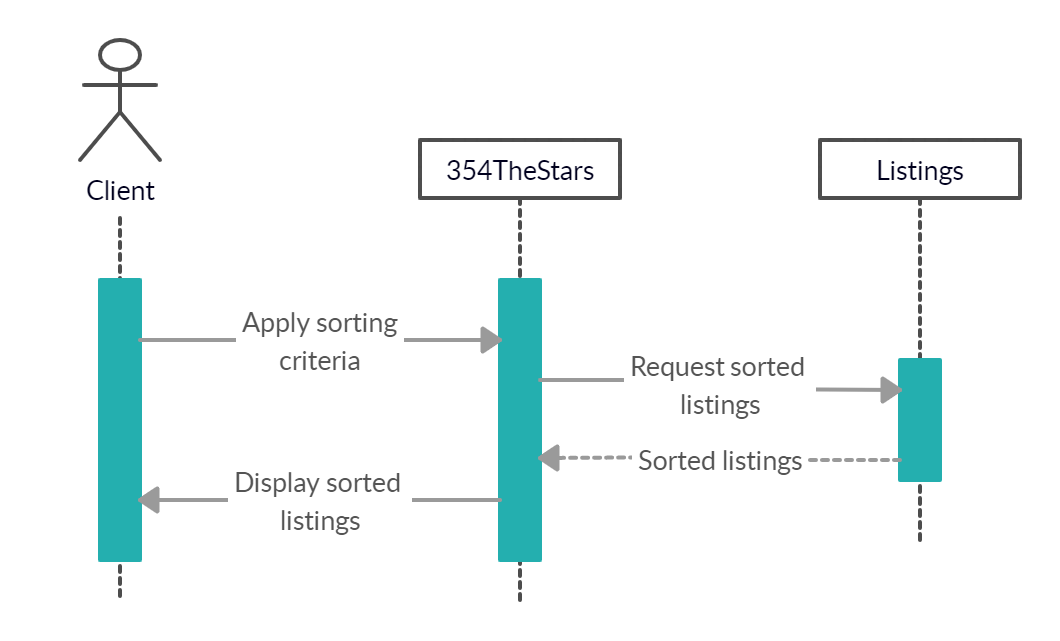
\includegraphics[width=0.6\textwidth,height=0.2\paperheight]{Diagrams/Sequence/Sort_Listings.jpg}
    \caption{Sequence Diagram 15: Sort Listings results}
    \label{fig: Sort Listings Results}
    \begin{justify}
        The client starts by applying a sorting criteria to the list of listings. The website then takes these sorting parameters and uses them to query the Listings table in the database. The sorted listings is then retrieved from the database and displayed to the client.
    \end{justify}
\end{figure}
\clearpage

\section{External Interface}

\begin{figure}[ht!]
    \subsection{Home Page}
    \centering
    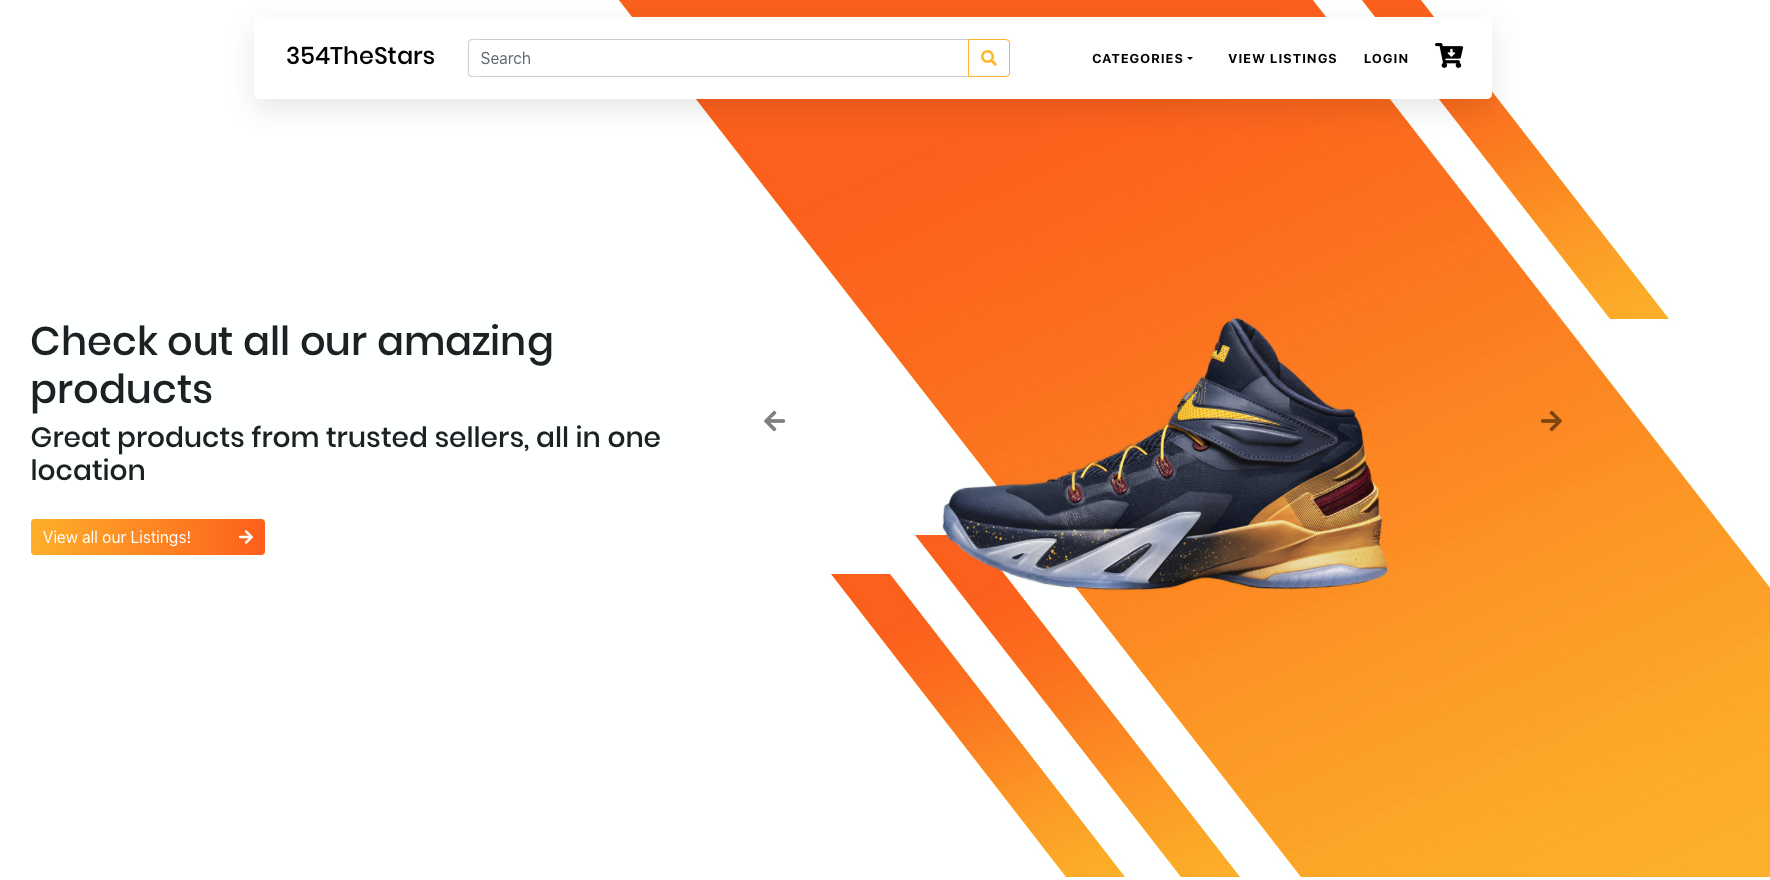
\includegraphics[width=\textwidth,height=0.3\paperheight,keepaspectratio]{Diagrams/External_Interfaces/Home_Page.png}
    \caption{Home Page}
    \label{fig: Home Page}
\end{figure}
\FloatBarrier


\begin{figure}[ht!]
    \subsection{Login}
    \centering
    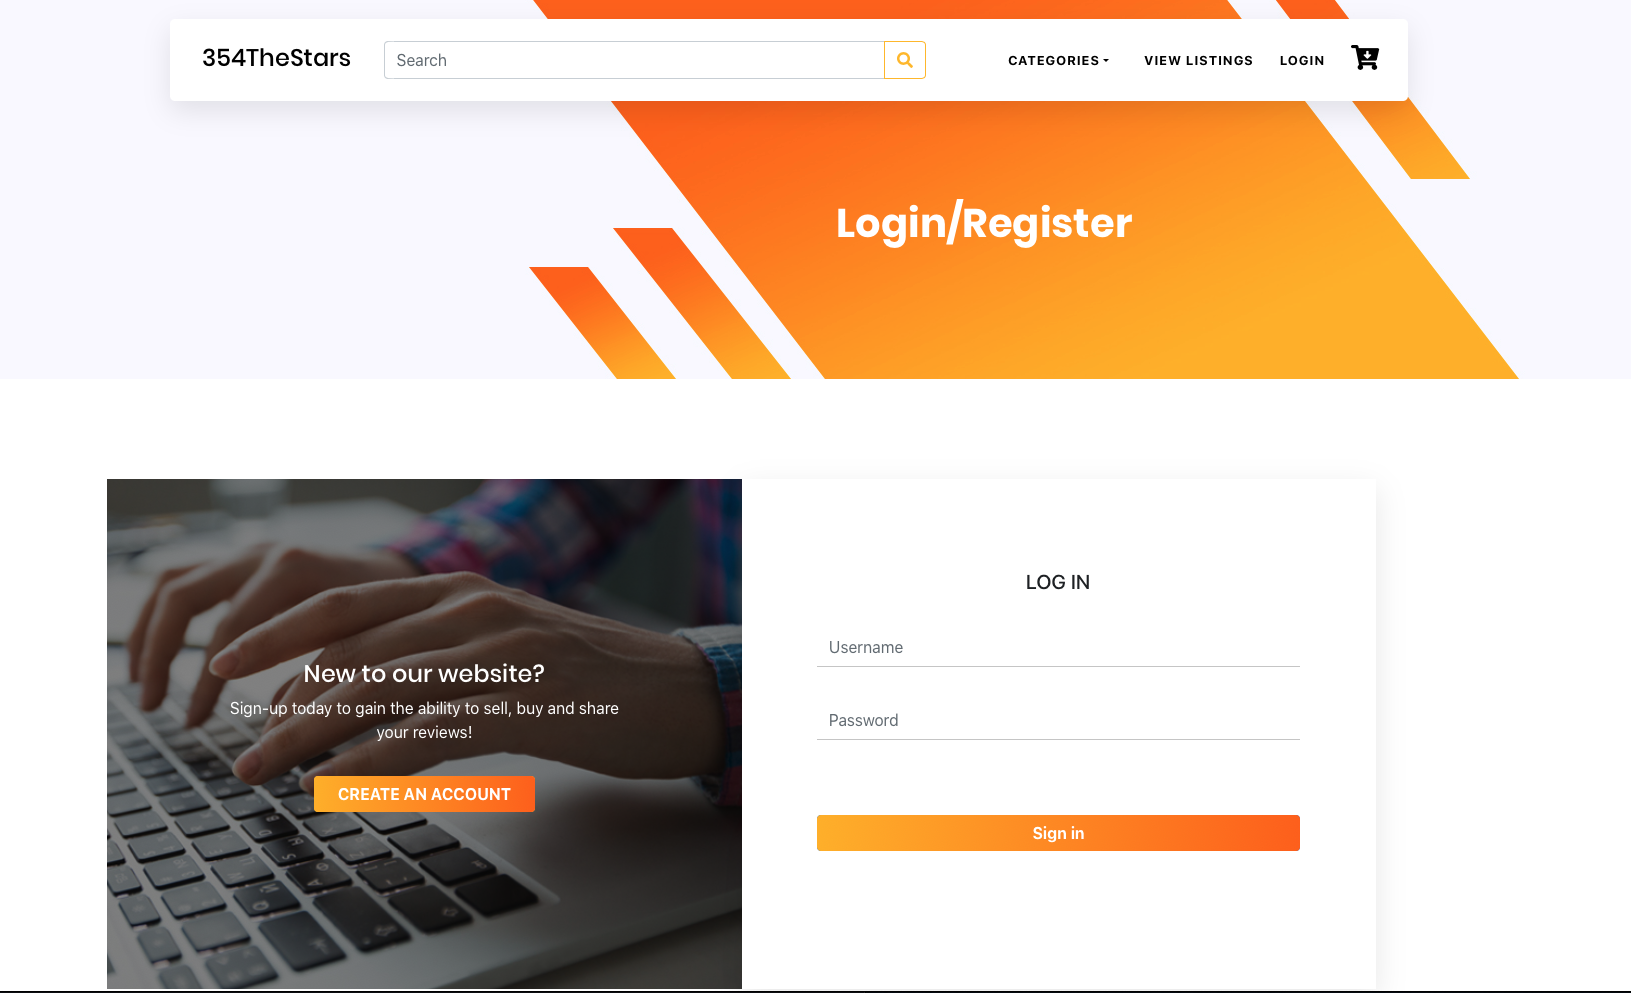
\includegraphics[width=\textwidth,height=0.3\paperheight,keepaspectratio]{Diagrams/External_Interfaces/Login.png}
    \caption{Login page}
    \label{fig: Login Page}
\end{figure}
\FloatBarrier


\begin{figure}[ht!]
    \subsection{Create account}
    \centering
    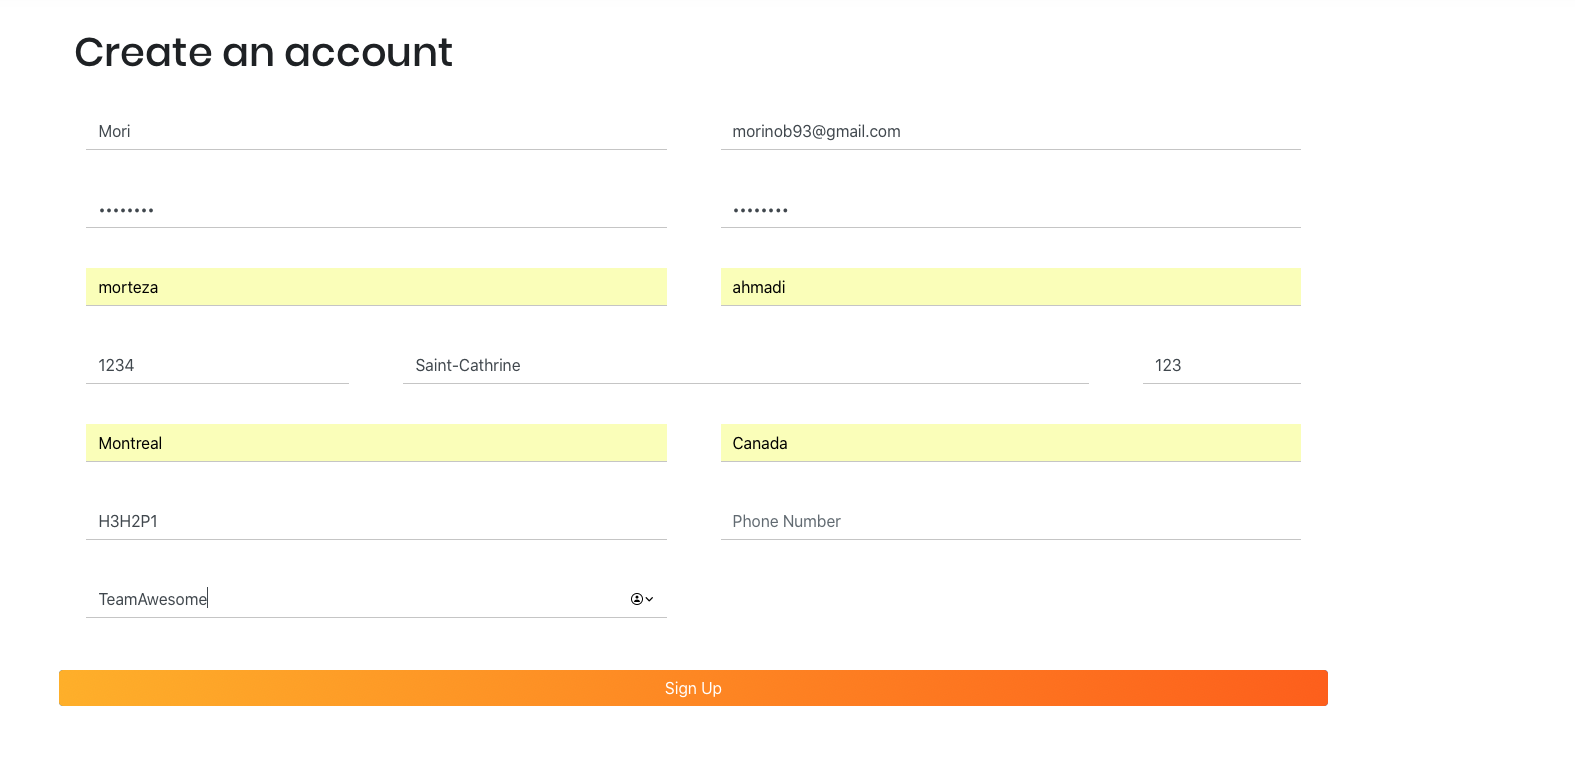
\includegraphics[width=\textwidth,height=0.3\paperheight,keepaspectratio]{Diagrams/External_Interfaces/Create_Account.png}
    \caption{Create Account Page}
    \label{fig: Create Account Page}
\end{figure}
\FloatBarrier


\begin{figure}[ht!]
    \subsection{Result of a category}
    \centering
    \includegraphics[width=\textwidth,height=3\paperheight,keepaspectratio]{Diagrams/External_Interfaces/Categories.png}
    \caption{Result of shoes category}
    \label{fig: Result of a category}
\end{figure}
\FloatBarrier


\begin{figure}[ht!]
    \subsection{Apply filters}
    \centering
    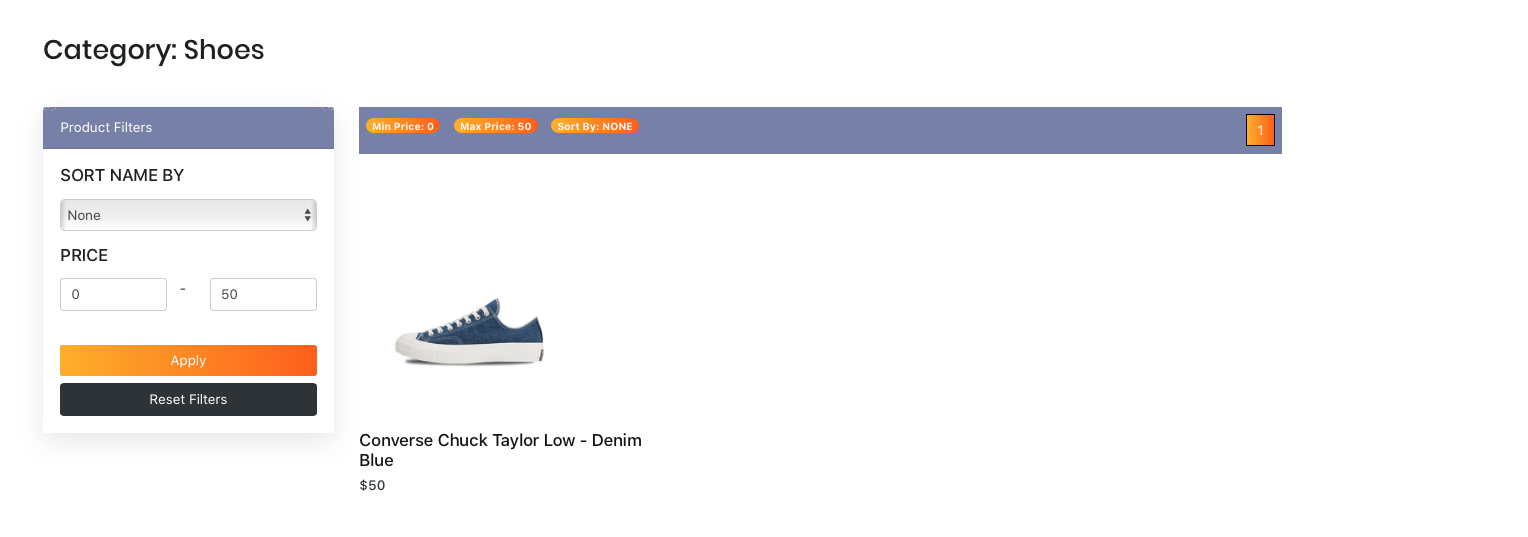
\includegraphics[width=\textwidth,height=0.3\paperheight,keepaspectratio]{Diagrams/External_Interfaces/Categories_filtered.png}
    \caption{Result of shoes category after applying filters}
    \label{fig: Apply filters}
\end{figure}
\FloatBarrier


\begin{figure}[ht!]
    \subsection{Search for an item}
    \centering
    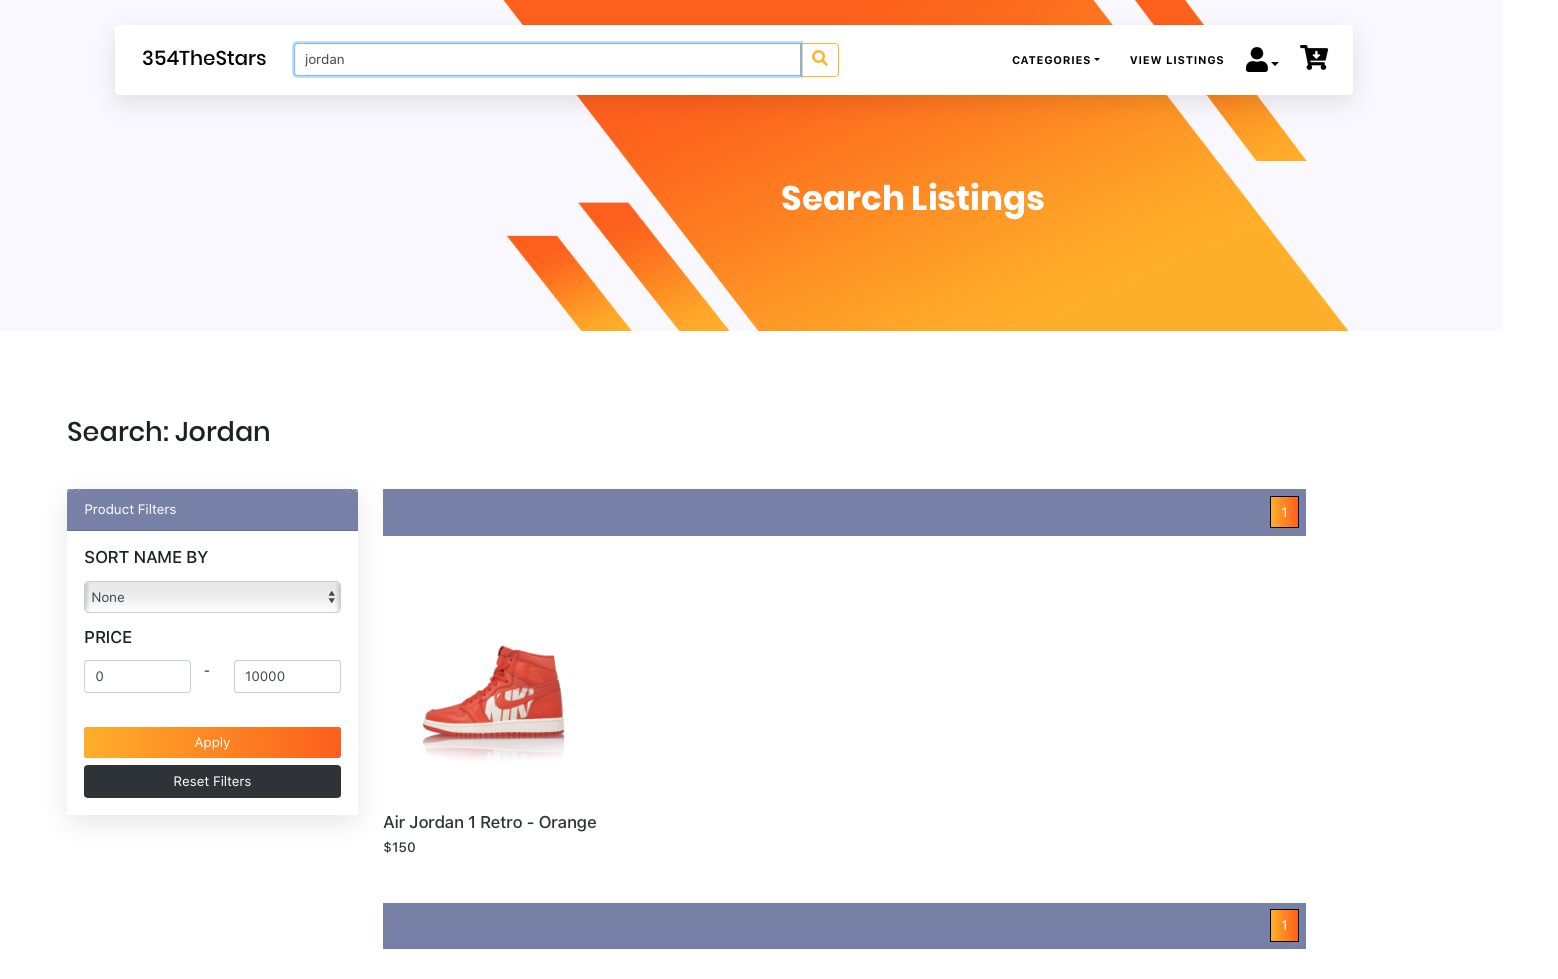
\includegraphics[width=\textwidth,height=0.3\paperheight,keepaspectratio]{Diagrams/External_Interfaces/Search_Listing.png}
    \caption{Search Results for query of "Jordan"}
    \label{fig: Search For An Item}
\end{figure}
\FloatBarrier

\begin{figure}[ht!]
    \subsection{List of listings}
    \centering
    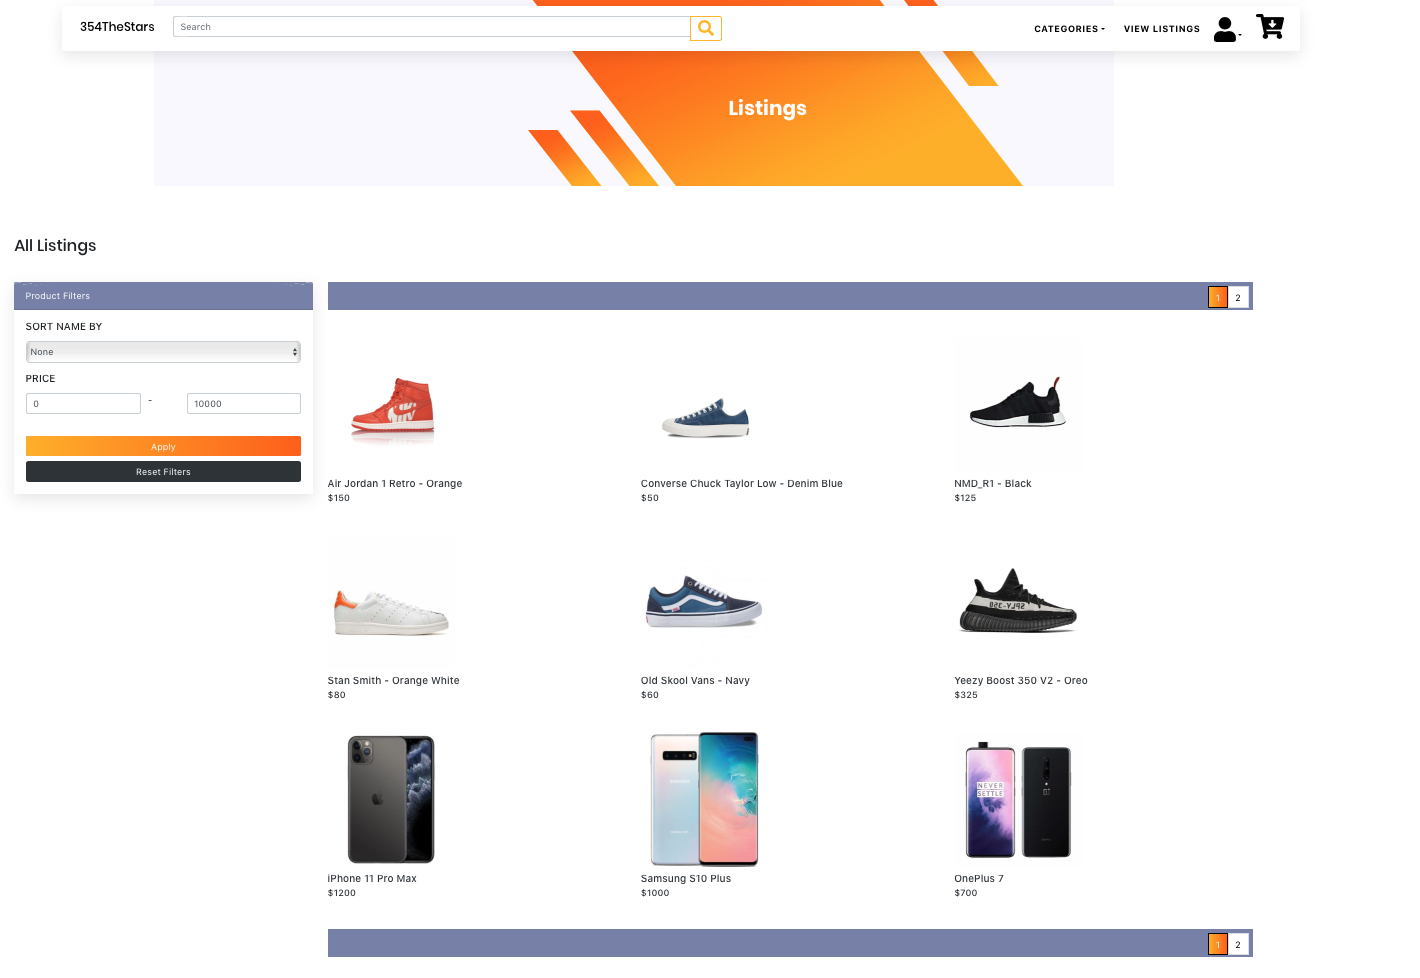
\includegraphics[width=\textwidth,height=0.3\paperheight,keepaspectratio]{Diagrams/External_Interfaces/List_Of_Listings_1.png}
    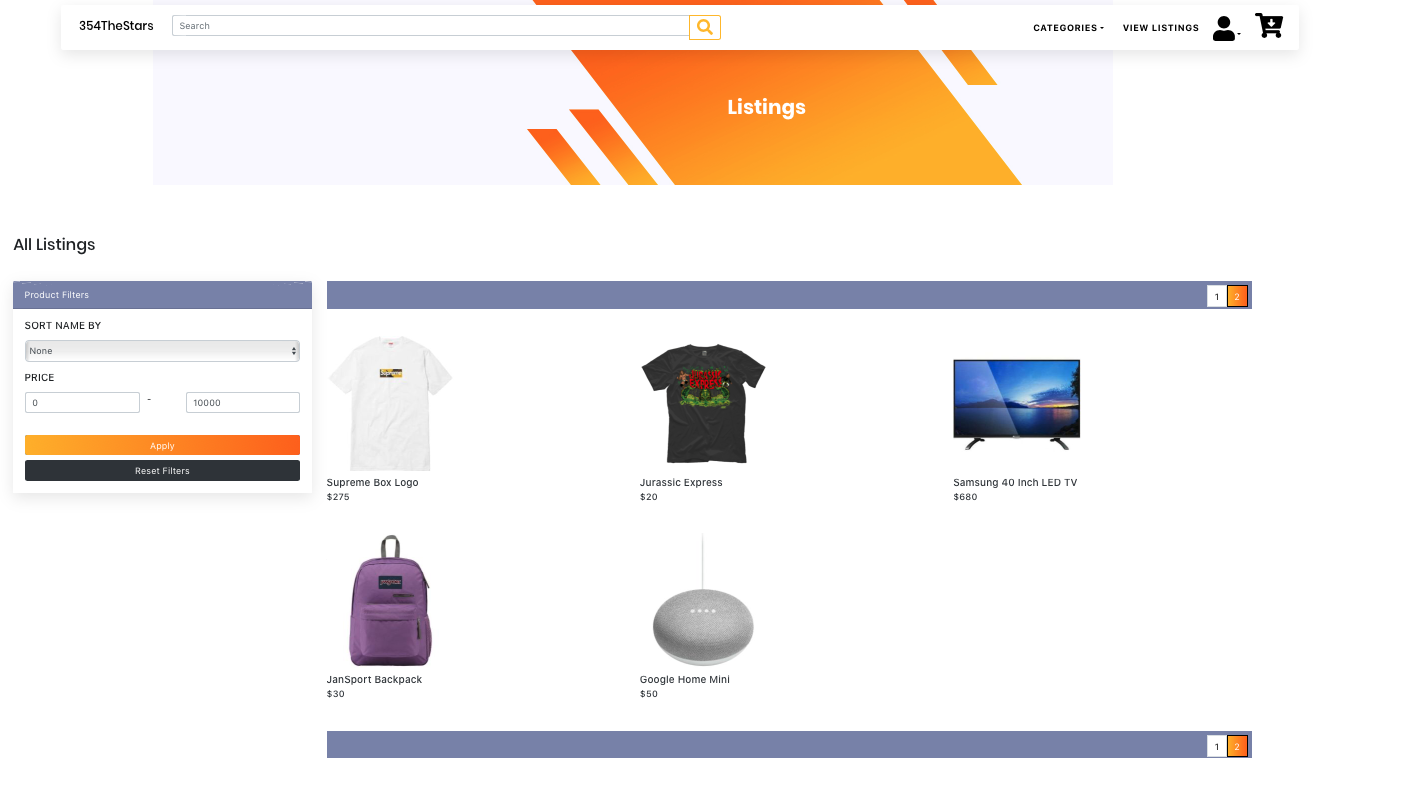
\includegraphics[width=\textwidth,height=0.3\paperheight,keepaspectratio]{Diagrams/External_Interfaces/List_Of_Listings_2.png}
    \caption{Paginated list of listings}
    \label{fig: List of listings}
\end{figure}

\FloatBarrier

\begin{figure}[ht!]
    \subsection{Latest listings}
    \centering
    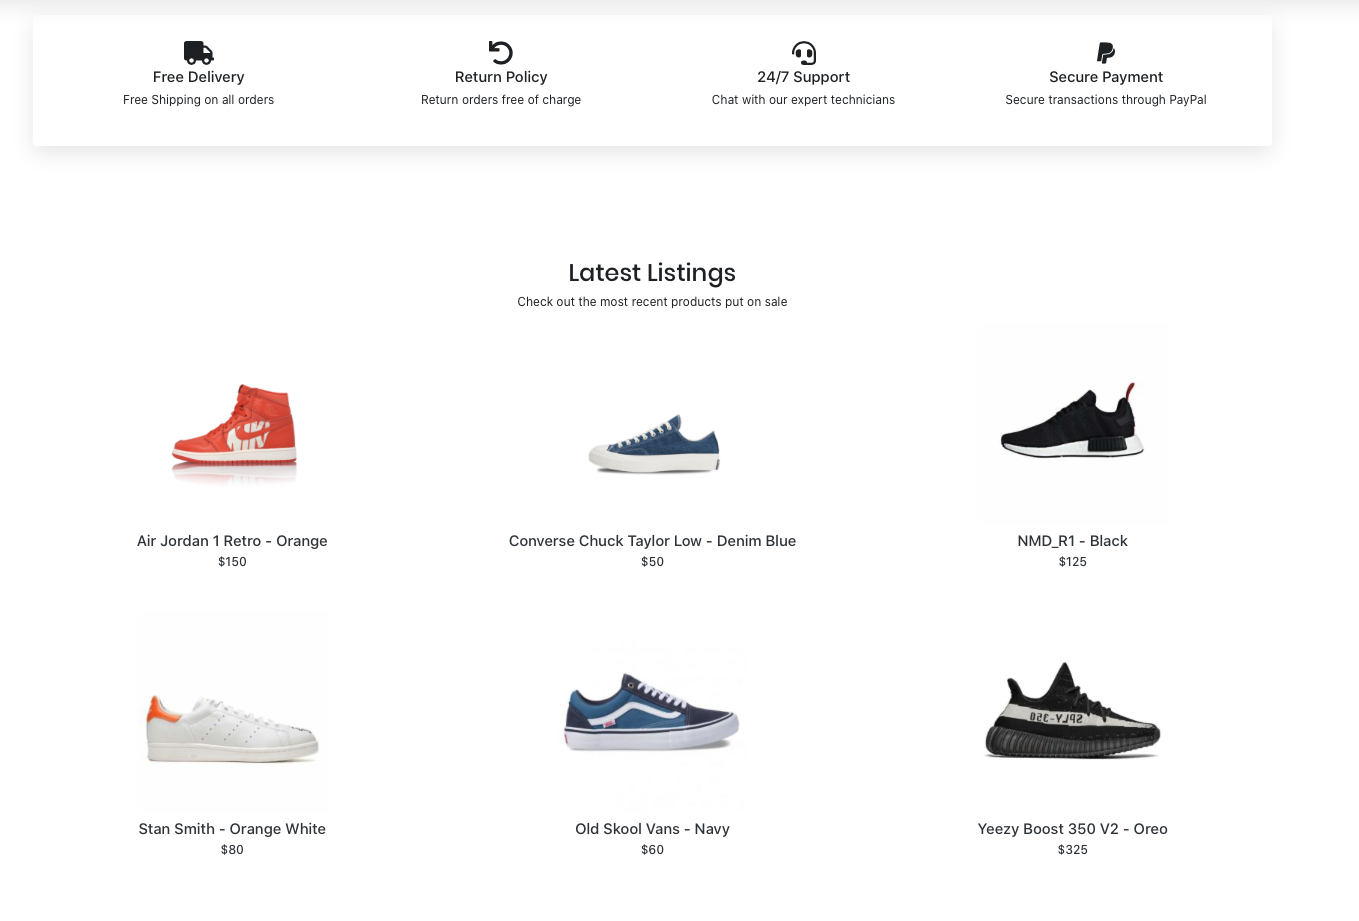
\includegraphics[width=\textwidth,height=0.3\paperheight,keepaspectratio]{Diagrams/External_Interfaces/Latest_Listings.png}
    \caption{Latest listing on home page}
    \label{fig: Latest listings}
\end{figure}
\clearpage

\section{Architectural Diagram}
\begin{figure}[ht!]
    \centering
    \includegraphics[width=\textwidth,height=0.6\paperheight]{Diagrams/Class/Architectural_diagram.png}
    \caption{Architectural Diagram}
    \label{fig: Architectural Diagram}
\end{figure}
\section{Tools and languages used}
    \subsection{Front-end}
        The front-end on the 354TheStars uses \textit{React} as the main framework for building the user interfaces as it is optimal for fetching rapidly changing data that needs to be recorded. We don't like how Javascript does not have any type checking so \textit{Typescript} saves us from a lot of trouble.
        The front-end also uses the \textit{react-router-dom} framework for a simple and easy way to handle routing to send requests to the back-end. 
        Front-end is all about the looks, and design. We achieved an attractive look by using  \textit{React-Bootstrap}  which provides design templates for user interface components. \textit{SASS} also helps us make beautiful styling for our UI components. 
        354TheStars provides minimalistic looking forms for a great user-experience. \textit{Formik} and \textit{Yup} help us in validating those forms.
    \subsection{Back-end}
        The back-end of 354TheStars uses \textit{Node.js} to provide a reliable server-side implementation. Since routing is a crucial part of the back-end we use the \textit{Express.js} framework to abstract some work on the networking layer. 
        Our back-end is not useful without data, in order to make the process of querying the database easier we benefit from the \textit{typeorm} framework.
        Since storing images in SQL is not really efficient, we make use of the \textit{Cloudinary} framework which is a cloud-based image and video management system. Therefore, we achieve a faster and more efficient way of storing and fetching media.
        We want to have a fast and reliable contact with our users. For that reason we use \textit{NodeMailer} to send emails from the server to clients. This is used for the forgot-password feature.
    \subsection{Database}
        The 354TheStars uses relational database. For that reason, \textit{MySQL} is a good candidate. In order to have consistent data between all of your clients, a SQL server is required. We use the \textit{Google Cloud Platform} to have our SQL server.
\section{Glossary of Domain Concepts} \label{glossary}
\begin{table}[H]
    \caption{Glossary of Domain Concepts}
    \begin{center}
        \scalebox{0.7}{
            \begin{tabular}{|l|p{0.8\linewidth}|}
                \hline
                Expression &  Definition \\
                \hline
                \index{administrator}Admin & The person who manages the website as well as users and \index{product}products.  \\
                \hline
                User Account & A \index{data}data object containing user \index{information}information including username, email, address(es), phone number. \\
                \hline
                Registered User & The person who has successfully made a user account. \\
                \hline
                \index{guest user}Guest User & The person who is not a \index{registered user}registered user, however has the ability to browse the website. \\
                \hline
                \index{PayPal}PayPal & PayPal Holdings Inc. is an American company that operates a worldwide online \index{payment}payment platform. \\
                \hline
                Database & A local or online container which holds \index{data}data in an organised, efficient manner. \\
                \hline
                Server & A computer that is accessible on a network, on which a database and/or system may be hosted. The bank institutions' databases will be hosted on here. \\
                \hline
                \index{React}React & React is a JavaScript library for building user interfaces. It is maintained by Facebook and a community of individual developers and companies. \\
                \hline
                \index{Typescript}TypeScript & Typescript is an open-source programming language developed and maintained by Microsoft. It is a strict syntactical superset of JavaScript, and adds optional static typing to the language. \\
                \hline
                \index{React Router}React Router & React Router is a collection of navigational components that compose declaratively with your application. \\
                \hline
                \index{SASS}SASS & SASS (Syntactically Awesome Style Sheets) is an extension of CSS that enables you to use things like variables, nested rules, inline imports and more. It also helps to keep things organised and allows you to create style sheets faster. \\
                \hline
                \index{Formik}Formik & Formik is a small library that helps you with the 3 most annoying parts: Getting values in and out of form state. Validation and error messages. Handling form submission. \\
                \hline
                \index{Yup}Yup & Yup is a JavaScript object schema validator and object parser. \\
                \hline
                \index{Node.js}Node.js & Node.js run-time environment includes everything you need to run a program on your machine as a standalone application.\\
                \hline
                \index{Express.js}Express & Express is a light-weight web application framework to help organize your web application into an MVC architecture on the server side. \\
                \hline 
                \index{ORM}ORM & Object-relational mapping (ORM, O/RM, and O/R mapping tool) in computer science is a programming technique for converting data between incompatible type systems using object-oriented programming languages. \\
                \hline
                \index{Typeorm}TypeORM & TypeORM is an ORM that can run in NodeJS, Browser, Cordova, PhoneGap, Ionic, React Native, NativeScript, Expo, and Electron platforms and can be used with TypeScript and JavaScript. \\
                \hline 
                \index{Cloudinary}Cloudinary & Cloudinary is the market leader in providing a comprehensive cloud-based image and video management platform. \\
                \hline
                \index{SQL}SQL & SQL (pronounced "ess-que-el") stands for Structured Query Language. SQL is used to communicate with a database.  \\
                \hline
                \index{MySQL}MySQL & MySQL is a freely available open source Relational Database Management System (RDBMS) that uses Structured Query Language (SQL). \\
                \hline
            \end{tabular}}
    \end{center}
\end{table}
\section{Conclusion}

With the continued evolution of technology, shoppers are moving away from retail
and embracing e-commerce sites. This is where 354TheStars comes in, which provides
a space for businesses and individuals to shop and/or sell all series of products
while they are home, at work, commuting, or from anywhere in the world as long
as they connect with a device and an internet connection. 354TheStars will bring
shoppers together as they review the products they have received with 354TheStars'
incredible shipping time, and share their experiences on the platform. With a
simple mission and a clear vision for what an e-commerce site should be, 354TheStars
is set to attract a great number of individuals and businesses.

\appendix
\section{Final Requirements}
\begin{itemize}
    \item \textbf{Sell:} The system allows a registered user to add \index{product}product and its details (price, description, image) to be able to sell the product.
    \item \textbf{Buy:} The system allows a \index{registered user}registered user to buy a product. Also the \index{buyer}buyer can \index{review}review the purchased product after fifteen days.
    \item \textbf{Search:} The system allows both a registered user and \index{guest user}guest user to browse and search through all the \index{product}products.
    \item \textbf{Admin panel:} The \index{administrator}admin panel allows the admin to manage, view, and edit user accounts and their \index{information}information such as (username, email, address, phone number). The panel also allows the admin to manage, view and edit all the products in the website.
    \item \textbf{Purchase process:} The system provides a secure and safe online \index{payment}payment system for \index{buyer}buyers. They can use their \index{PayPal}PayPal account to buy \index{product}products from the website.
    \item \textbf{Advertisements:} The system should display items which are cheap and attractive or with different variety on the home page while keeping it attractive. It also should display advertisements with help of cookies.
    \item \textbf{Commision on sales:} The system should get 3\% for the first 10 sold items. 8\% for the rest of items, also seller can not sell items for free.
    \item \textbf{Search and Filter:} The system should allow users to search for any items by name, and filters should be implemented to improve User Interface.
    \item \textbf{Reviews:} Sellers can not remove any reviews on their product, but they can reply to reviews (One reply per review).
    \item \textbf{Security: } The system should encrypte passwords then store in database.
    \item \textbf{Forgot password:} The system should allow users to reset their password, in case they forget their password.
    \item \textbf{Updating cart:} The system should allow users to edit their cart by letting them to add or delete a listing.
\end{itemize}

\section{Index}

\printindex


\section{Reference}

\begin{itemize}
    \item User information: As our user and use-cases was based on feedback provided by our developers, our references lie mainly within our own team.
    \item Hakim Mellah's course COMP 354 content
    \item Ian Sommerville, Software Engineering. 10 Edition
    \item Roger S. Pressman, Software Engineering: a Practitioner's Approach, 7th edition
    \item Description of Formik from https://www.npmjs.com/package/formik
    \item Description of Yup from https://www.npmjs.com/package/Yup
    \item What is SASS? from https://www.creativebloq.com
    \item What exactly is Node.js? https://www.freecodecamp.org/
    \item What is Express js? https://stackoverflow.com/questions/12616153/what-is-express-js
    \item Description of Typeorm from https://www.npmjs.com/package/typeorm
    \item About Cloudinary from https://cloudinary.com/about
    \item About MySQL from https://www.mysql.com/about/
\end{itemize}
\end{document}
